\documentclass[14pt,aspectratio=169]{beamer}
\usetheme{default}
% something tries to renewcommand these but beamer must break the assumption that they are defined so I am defining them
\newcommand{\labelitemi}{}
\newcommand{\labelitemii}{}
\newcommand{\labelitemiii}{}
\newcommand{\labelitemiv}{}
\renewcommand{\mathrm}[1]{\mathsf{#1}}
\usepackage{greg}
\renewcommand{\defemph}[1]{\alert{#1}}
\useoutertheme[subsection=false]{miniframes}
\useinnertheme{circles}
\setbeamertemplate{navigation symbols}{}
\setbeamercovered{transparent}
\definecolor{cmu_red}{RGB}{176,28,51} % #990000
\definecolor{cmu_dark_grey}{RGB}{70, 70, 70} % #464646
\definecolor{mygrey}{RGB}{100, 100, 100}
\definecolor{steveblue}{RGB}{51, 51, 172}
\usecolortheme[named=cmu_red]{structure}
\setbeamercolor{palette secondary}{bg=steveblue,fg=white}
\setbeamercolor{palette tertiary}{bg=steveblue,fg=white}
\setbeamercolor{section in head/foot}{bg=mygrey,fg=white}
\setbeamercolor{alerted text}{fg=cmu_red}

% \setbeamercolor{corollary title}{use=structure,fg=white,bg=structure.fg!75!black}
% \setbeamercolor{corollary body}{parent=normal text,use=block title,bg=blue}
%\setlength{\parskip}{\baselineskip} 

\commentout{
The thesis reads like this:
The type of torsors and Eilenberg-Mac Lane spaces is the background in HoTT of our theory. 
Manifolds are simplicial complexes, made into pushouts in an obvious way, with hubs and spokes.
Extending a map from the k-skel to the (k+1)-skel is called a connection.
Extending a map to a single face is a flatness structure.
Focus on 2-dimensions, oriented, tangent bundles:
Vector fields! Sections on the 1-skel.
Vector fields do the ice cream scoop thing to paths.
Index on a face: swirling after factoring in the flatness.
Flatness and index on two faces.
}

\title[Geometry in HoTT]{DRAFT: Discrete differential geometry in homotopy type theory}
\author{Greg Langmead}
\institute[CMU]{Carnegie Mellon University}
\logo{\vspace{-4pt}
\includegraphics[width=100pt]{figs/cmu-wordmark-horizontal-r.pdf}\quad}
\date{April 2025}

\begin{document}
\begin{frame}
\titlepage
\end{frame}

% \begin{frame}
% \tableofcontents
% \end{frame}

\section{Motivation}

\begin{frame}{Motivation}
To use HoTT to study \alert{connections} and \alert{explain} their applicability to algebraic topology, via
\begin{itemize}
\item the Gauss-Bonnet theorem
\item its vast generalization, Chern-Weil theory
\end{itemize}
\end{frame}

\begin{frame}
\begin{theorem}[Gauss-Bonnet]
Let \( M \) be a compact 2-manifold without boundary, equipped with a Riemannian metric. Let \( K \) be the Gaussian curvature of \( M \) and let \( \chi(M) \) be the Euler characteristic. Then \[\frac{1}{2\pi}\int_M K\,dA=\chi(M).\]
\end{theorem}
\end{frame}

\begin{frame}
\vspace{10pt}\begin{theorem}[Poincaré-Hopf]
Let \( M \) be a compact smooth manifold without boundary. Let \( X \) be a vector field on \( M \) with isolated zeroes \( x_1,\ldots,x_n \). Then \[\sum_{i=1}^{n} \mathsf{index}_{x_i}=\chi(M).\]
\end{theorem}
\vspace{-40pt}
% RADIAL OUTWARD
\begingroup
\colorlet{veccol}{cmu_red}
\colorlet{myblue}{blue!60!black}
\tikzstyle{vector}=[->,thick,veccol,style={-{Stealth[scale=0.9]}}]
\pgfmathsetmacro{\R}{1}%
\pgfmathsetmacro{\r}{0.03}%
\pgfmathsetmacro{\N}{8}%
\pgfmathsetmacro{\ang}{60}%
\pgfmathsetmacro{\RR}{0.5}%
\[
% zero
\onslide<1->{
\begin{tikzpicture}
  \fill[myblue] (0,0) circle (\r);
  \foreach \x/\y in {-1/0,-1/1,0/1,1/1,1/0,-1/-1,0/-1,1/-1}{
    \draw[vector] (\x*0.5*\R,\y*0.5*\R) ++ (\ang-180:\R/2) --++ (\ang:\R);
  }
  \node at (0,-1.35*\R) {index 0};
\end{tikzpicture}}
\onslide<1->{
% outward
\begin{tikzpicture}
  \fill[myblue] (0,0) circle (\r);
  \foreach \i [evaluate={\ang=\i*360/\N;}] in {0,...,\N}{
    \draw[vector] (\ang:0.1*\R) --++ (\ang:\R);
  }
  \node at (0,-1.35*\R) {index +1};
\end{tikzpicture}
% inward
\begin{tikzpicture}
  \fill[myblue] (0,0) circle (\r);
  \foreach \i [evaluate={\ang=\i*360/\N;}] in {0,...,\N}{
    \draw[vector] (\ang:1.1*\R) -- (\ang:0.1*\R);
  }
  \node at (0,-1.35*\R) {index +1};
\end{tikzpicture}
% counterclock
\begin{tikzpicture}
  \fill[myblue] (0,0) circle (\r);
  \foreach \R in {0.44,0.88}{
    \foreach \i [evaluate={\ang=\i*360/\N;}] in {1,...,\N}{
      \draw[vector] (\ang:\R) --++ (\ang+90:\RR);
    }
  }
  \node at (0,-1.3*\R) {index +1};
\end{tikzpicture}
% clockwise
\begin{tikzpicture}
  \fill[myblue] (0,0) circle (\r);
  \foreach \R in {0.44,0.88}{
    \foreach \i [evaluate={\ang=\i*360/\N;}] in {1,...,\N}{
      \draw[vector] (\ang:\R) --++ (\ang-90:\RR);
    }
  }
  \node at (0,-1.3*\R) {index +1};
\end{tikzpicture}}
\onslide<1->{
% minus one
\pgfmathsetmacro{\r}{0.03}%
\pgfmathsetmacro{\N}{20}%
\pgfmathsetmacro{\ang}{10}%
\begin{tikzpicture}
  \fill[myblue] (0,0) circle (\r);
  \foreach \R in {0.88}{
    \foreach \i [evaluate={\ang=\i*360/\N;}] in {1,...,\N}{
      \draw[vector] (\ang:\R) --++ (-\ang-90:\RR);
    }
  }
  \node at (0,-1.3*\R) {index --1};
\end{tikzpicture}}
\]
\endgroup
% \includegraphics[width=420pt]{figs/needham_indexes.pdf}
\end{frame}

% \begin{frame}
% I was guided by these pseudo-methods:
% \begin{itemize}
% \item<2-> Infinitesimals are not core to differential geometry
% \item<3-> The action on paths \( \ap f \) is the derivative of \( f \)
% \item<4-> HoTT transport is parallel transport
% \end{itemize}
% \onslide<5->{and therefore}
% \begin{itemize}
% \item<6-> A connection is a derivative of a classifying map: a choice of connection on a bundle \( P:M\to\uni \) is a choice of action on paths
% \end{itemize}
% \onslide<7->{How can this be? The derivative of \( f \) is calculated from the data of \( f \), it's not a free choice!}
% \end{frame}

\begin{frame}{Plan}
\begin{itemize}
\item Manifolds
\item Classifying maps
\item Connections and curvature
\item Theorems
\end{itemize}
\end{frame}

\begin{frame}{HoTT background}
\begin{enumerate}
\item Bezem,~M., Buchholtz,~U., Cagne,~P., Dundas,~B.~I., and Grayson,~D.~R.,
  (2021-) Symmetry. \url{https://github.com/UniMath/SymmetryBook}.

\item Buchholtz,~U., Christensen,~J.~D. , Flaten,~J.~G.~T., and Rijke,~E. (2023) Central
  H-spaces and banded types. arXiv:2301.02636

\item Scoccola,~L. (2020) Nilpotent types and fracture squares in homotopy type theory, MSCS 30(5). arXiv:1903.03245
\end{enumerate}
\end{frame}

\section{Discrete manifolds}

\begin{frame}{Discrete manifolds in HoTT}
\begin{itemize}
\item Recall the classical theory of \alert{simplicial complexes}
\item Define a \alert{realization} procedure to turn them into homotopy pushouts
\end{itemize}
\end{frame}

\begin{frame}{Simplicial complexes}
\begin{mydef}
An \defemph{abstract simplicial complex \( M \) of dimension \( n \)} is an ordered list of sets \( M\defeq[M_0,\ldots,M_n] \) consisting of 
\begin{itemize}
\item a set \( M_0 \) of \( (n+1) \) vertices
\item sets \( M_k \) of subsets of \( M_0 \) of cardinality \( k+1 \)
\item downward closed: if \( F\in M_k \) and \( G\subseteq F \), \( |G|=j+1 \) then \( G\in M_j \)
\end{itemize}
We call the truncated list \( M_{\leq k}\defeq [M_0,\ldots,M_k] \) \alert{the \( k \)-skeleton of \( M \)}.
\end{mydef}
\end{frame}

\begin{frame}{Simplicial complexes}
\begin{example}
The \defemph{complete simplex of dimension \( n \)}, denoted \( P(n), \) is the set \( \{1,\ldots,n+1\} \) and its power set. The \( (n-1) \)-skeleton \( P(n)_{\leq (n-1)} \) is denoted \alert{\( \partial P(n) \)} and will serve as a combinatorial \( (n-1) \)-sphere.
\end{example}
e.g., \( \partial P(2) \) is an abstract triangle with 3 vertices and 3 edges (lacks its face).
\end{frame}

\begin{frame}{Simplicial complexes}
\begin{columns}
\begin{column}{0.5\textwidth}
\!\!\!\!\!\vspace{-0.5cm}\resizebox{220pt}{!}{
\begin{tikzpicture}[scale=0.1]
    \matrix (A) [matrix of math nodes, row sep=1cm, column sep=-.2cm]
    { 
       ~ &  ~ & ~ & ~ & ~ & \left\{\substack{{w, b, r}\\ {g, o, y}}\right\} \\  
  ~ &  ~ & \scriptstyle\{w, b, r\} & \scriptstyle\{w, r, g\}  & \scriptstyle\{w, g, o\} & \scriptstyle\{w, o, b\} & \scriptstyle\{y, b, r\} & \scriptstyle\{y, r, g\}  & \scriptstyle\{y, g, o\} & \scriptstyle\{y, o, b\}\\
  \scriptstyle\{w, b\} & \scriptstyle\{w,r\}  & \scriptstyle\{w,g\} & \scriptstyle\{w,o\} & \scriptstyle\{b, r\} & \scriptstyle\{r, g\}  & \scriptstyle\{g, o\} & \scriptstyle\{o, b\} & \scriptstyle\{y, b\} & \scriptstyle\{y,r\}  & \scriptstyle\{y,g\} & \scriptstyle\{y,o\}\\
  ~ & ~ & ~ &  \scriptstyle\{w\}  & \scriptstyle\{b\} & \scriptstyle\{r\} & \scriptstyle\{g\} & \scriptstyle\{o\} & \scriptstyle\{y\}\\
      ~ & ~ &  ~ & ~ & ~ & \emptyset \\
    };
    \draw (A-1-6.south)--(A-2-3.north);
    \draw (A-1-6.south)--(A-2-4.north);
    \draw (A-1-6.south)--(A-2-5.north);
    \draw (A-1-6.south)--(A-2-6.north);
    \draw (A-1-6.south)--(A-2-7.north);
    \draw (A-1-6.south)--(A-2-8.north);
    \draw (A-1-6.south)--(A-2-9.north);
    \draw (A-1-6.south)--(A-2-10.north);

    \draw (A-2-3.south)--(A-3-1.north);
    \draw (A-2-3.south)--(A-3-2.north);
    \draw (A-2-3.south)--(A-3-5.north);

    \draw (A-2-4.south)--(A-3-2.north);
    \draw (A-2-4.south)--(A-3-3.north);
    \draw (A-2-4.south)--(A-3-6.north);

    \draw (A-2-5.south)--(A-3-3.north);
    \draw (A-2-5.south)--(A-3-4.north);
    \draw (A-2-5.south)--(A-3-7.north);

    \draw (A-2-6.south)--(A-3-4.north);
    \draw (A-2-6.south)--(A-3-1.north);
    \draw (A-2-6.south)--(A-3-8.north);

    \draw (A-2-7.south)--(A-3-5.north);
    \draw (A-2-7.south)--(A-3-10.north);
    \draw (A-2-7.south)--(A-3-9.north);

    \draw (A-2-8.south)--(A-3-6.north);
    \draw (A-2-8.south)--(A-3-11.north);
    \draw (A-2-8.south)--(A-3-10.north);

    \draw (A-2-9.south)--(A-3-7.north);
    \draw (A-2-9.south)--(A-3-12.north);
    \draw (A-2-9.south)--(A-3-11.north);

    \draw (A-2-10.south)--(A-3-8.north);
    \draw (A-2-10.south)--(A-3-9.north);
    \draw (A-2-10.south)--(A-3-12.north);

    \draw (A-3-1.south)--(A-4-4.north);
    \draw (A-3-1.south)--(A-4-5.north);

    \draw (A-3-2.south)--(A-4-4.north);
    \draw (A-3-2.south)--(A-4-6.north);

    \draw (A-3-3.south)--(A-4-4.north);
    \draw (A-3-3.south)--(A-4-7.north);

    \draw (A-3-4.south)--(A-4-4.north);
    \draw (A-3-4.south)--(A-4-8.north);

    \draw (A-3-5.south)--(A-4-5.north);
    \draw (A-3-5.south)--(A-4-6.north);

    \draw (A-3-6.south)--(A-4-6.north);
    \draw (A-3-6.south)--(A-4-7.north);

    \draw (A-3-7.south)--(A-4-7.north);
    \draw (A-3-7.south)--(A-4-8.north);

    \draw (A-3-8.south)--(A-4-8.north);
    \draw (A-3-8.south)--(A-4-5.north);

    \draw (A-3-9.south)--(A-4-9.north);
    \draw (A-3-9.south)--(A-4-5.north);

    \draw (A-3-10.south)--(A-4-9.north);
    \draw (A-3-10.south)--(A-4-6.north);

    \draw (A-3-11.south)--(A-4-9.north);
    \draw (A-3-11.south)--(A-4-7.north);

    \draw (A-3-12.south)--(A-4-9.north);
    \draw (A-3-12.south)--(A-4-8.north);

    \draw (A-4-4.south)--(A-5-6.north);
    \draw (A-4-5.south)--(A-5-6.north);
    \draw (A-4-6.south)--(A-5-6.north);
    \draw (A-4-7.south)--(A-5-6.north);
    \draw (A-4-8.south)--(A-5-6.north);
    \draw (A-4-9.south)--(A-5-6.north);

\end{tikzpicture}%
}
\resizebox{90pt}{!}{%
\begin{figure}[h]
\centering
\begin{tikzpicture}%
  [x={(-0.860769cm, -0.121512cm)},
  y={(0.508996cm, -0.205391cm)},
  z={(-0.000053cm, 0.971107cm)},
  scale=1,
  back/.style={loosely dotted, thin},
  edge/.style={black, thick},
  facet/.style={fill=blue!95!black,fill opacity=0.1},
  vertex/.style={inner sep=1pt,circle,draw=green!25!black,fill=black,thick}]
\coordinate (-1, -1, 0) at (-1, -1, 0);
\coordinate (-1, 1, 0) at (-1, 1, 0);
\coordinate (0, 0, -1) at (0, 0, -1);
\coordinate (0, 0, 1) at (0, 0, 1);
\coordinate (1, -1, 0) at (1, -1, 0);
\coordinate (1, 1, 0) at (1, 1, 0);
%% Drawing edges in the back
%%
\draw[edge,back] (-1, -1, 0) -- (-1, 1, 0);
\draw[edge,back] (-1, -1, 0) -- (0, 0, -1.4);
\draw[edge,back] (-1, -1, 0) -- (0, 0, 1.4);
\draw[edge,back] (-1, -1, 0) -- (1, -1, 0);
%% Drawing vertices in the back
%%
\node[vertex] at (-1, -1, 0)     {};
%% Drawing the facets
%%
\fill[facet] (1, 1, 0) -- (0, 0, -1.4) -- (1, -1, 0) -- cycle {};
\fill[facet] (1, 1, 0) -- (0, 0, 1.4) -- (1, -1, 0) -- cycle {};
\fill[facet] (1, 1, 0) -- (-1, 1, 0) -- (0, 0, 1.4) -- cycle {};
\fill[facet] (1, 1, 0) -- (-1, 1, 0) -- (0, 0, -1.4) -- cycle {};
%% Drawing edges in the front
%%
\draw[edge] (-1, 1, 0) -- (0, 0, -1.4);
\draw[edge] (-1, 1, 0) -- (0, 0, 1.4);
\draw[edge] (-1, 1, 0) -- (1, 1, 0);
\draw[edge] (0, 0, -1.4) -- (1, -1, 0);
\draw[edge] (0, 0, -1.4) -- (1, 1, 0);
\draw[edge] (0, 0, 1.4) -- (1, -1, 0);
\draw[edge] (0, 0, 1.4) -- (1, 1, 0);
\draw[edge] (1, -1, 0) -- (1, 1, 0);
%% Drawing the vertices in the front
%%
\begin{scope}[nodes=vertex]
\node[label=above right:\( b \)] at (-1, 1, 0)     {};
\node[label=below:\( y \)] at (0, 0, -1.4)     {};
\node[label=above:\( w \)] at (0, 0, 1.4)     {};
\node[label=above left:\( g \)] at (1, -1, 0)     {};
\node[label=above left:\( r \)] at (1, 1, 0)     {};
\node[label=above right:\( o \)] at (-1, -1, 0)     {};
\end{scope}
\end{tikzpicture}
\caption{The HIT \( \oo \) which has 6 points, 12 1-paths, 8 2-paths.}
\end{figure}

}
\quad
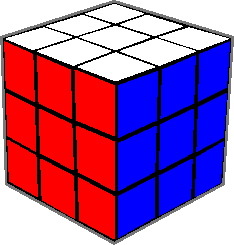
\includegraphics[width=60pt]{figs/hungarian_cube.pdf}
\end{column}
\begin{column}{0.5\textwidth}
Here is a \alert{Hasse diagram} of an abstract octahedron (vertices named for the colors on a Hungarian Cube)
\end{column}
\end{columns}
\end{frame}

\begin{frame}{Homotopy realization}
We will \alert{realize} simplicial complexes as pushouts.

The realization of a 0-dimensional complex \( M_0 \) is the set \( M_0 \).

In particular the 0-sphere \( \partial\Delta^1\defeq \partial P(1) \).
\end{frame}

\begin{frame}{Homotopy realization}
For a 1-dim complex \( M\defeq [M_0,M_1] \) form
\[% https://q.uiver.app/#q=WzAsNCxbMCwxLCJNXzA9XFxtYXRoYmJ7TX1fMCJdLFsxLDEsIlxcbWF0aGJie019XzEiXSxbMSwwLCJNXzEiXSxbMCwwLCJNXzFcXHRpbWVzIFxcYmRzaW1wbGV4bnsxfSJdLFswLDFdLFszLDAsIlxcbWF0aGJie0F9XzAiLDJdLFszLDIsIlxcbWF0aHJte3ByfV8xIl0sWzIsMSwiKl97XFxtYXRoYmJ7TX1fMX0iXSxbMSwzLCIiLDIseyJvZmZzZXQiOjMsInN0eWxlIjp7Im5hbWUiOiJjb3JuZXItaW52ZXJzZSJ9fV0sWzAsMiwiaF8xIiwyLHsic2hvcnRlbiI6eyJzb3VyY2UiOjQwLCJ0YXJnZXQiOjQwfSwibGV2ZWwiOjJ9XV0=
\begin{tikzcd}
  {M_1\times \bdsimplexn{1}} & {M_1} \\
  {M_0=\mathbb{M}_0} & {\mathbb{M}_1}
  \arrow["{\mathrm{pr}_1}", from=1-1, to=1-2]
  \arrow["{\mathbb{A}_0}"', from=1-1, to=2-1]
  \arrow["{*_{\mathbb{M}_1}}", from=1-2, to=2-2]
  \arrow["{h_1}"', shorten <=14pt, shorten >=14pt, Rightarrow, from=2-1, to=1-2]
  \arrow[from=2-1, to=2-2]
  \arrow["\ulcorner"{pos=0, rotate=180}, shift left=1, draw=none, from=2-2, to=1-1]
\end{tikzcd}

\]
\[\{\{w\}, \{g\}\}\leftarrow \{\{w, g\}\}\times\{0, 1\}\to \{\{w, g\}\}\]
\end{frame}

% \begin{frame}{Homotopy realization}
% \vspace{5pt}\begin{definition}
% An \defemph{\( n \)-gon} \( \ccc(n) \) is the realization of a complex \( C(n) \):
% \begin{align*}
% C(n)_0 &= \{v_1,\ldots,v_n\} \\
% C(n)_1 &= \{e_1=\{v_1,v_2\}, \ldots, e_{n-1}=\{v_{n-1}, v_n\}, e_n=\{v_n, v_0\}\}
% \end{align*}
% \end{definition}
% \vspace{-15pt}Toss in two non-complexes \vspace{-20pt}
% \[ \ccc(1)\defeq S^1,\quad \ccc(2)\defeq \begin{tikzpicture}[scale=0.5, baseline=3.5mm]
% \tikzset{arrow/.style={-{Stealth[scale=1.1]}}}
% \tikzset{oo/.style={circle, scale=0.25, fill=black}}
% \tikzset{ooo/.style={circle, scale=0.25, fill=none}}
% \node[oo, label=above:\( v_1 \)] (V1) at (0, 2) {};
% \node[oo, label=below:\( v_2 \)] (V2) at (0, 0) {};
% \node[ooo] (V21) at (0.3, 1.75) {};
% \node[ooo] (V22) at (0.3, 0.25) {};
% \draw (V1) edge[bend right=60, swap, "\( \ell_{12} \)"] (V2);
% \draw (V1) edge[bend left=60, "\( r_{21} \)"] (V2);
% \end{tikzpicture}\]
% %We sometimes denote a polygon with vertices \( \{a, b, c\} \) with \( \gr{abc} \), its realization with \( \hgr{abc} \).
% \end{frame}

\begin{frame}
Next construct a 1-sphere \( \partial\Delta^2\defeq \)
\begin{tikzpicture}[baseline=3mm]
\tikzset{oo/.style={circle, scale=0.25, fill=black}}
\node[oo, label=left:\( a \)] at (-0.7, 0) (a) {};
\node[oo, label=right:\( b \)] at  (0, 1) (b) {};
\node[oo, label=right:\( c \)] at  (0.7, 0) (c) {};
\draw (a) -- (b);
\draw (b) -- (c);
\draw (c) -- (a);
\end{tikzpicture} as the realization of \( \partial P(2) \):
\[% https://q.uiver.app/#q=WzAsNCxbMSwwLCJcXHBhcnRpYWwgUCgyKV8xIl0sWzEsMSwiXFxwYXJ0aWFsXFxEZWx0YV4yIl0sWzAsMCwiXFxwYXJ0aWFsIFAoMilfMVxcdGltZXMgXFxwYXJ0aWFsXFxEZWx0YV4wIl0sWzAsMSwiXFxwYXJ0aWFsIFAoMilfMCJdLFsyLDBdLFsyLDNdLFszLDFdLFswLDFdLFsxLDIsIiIsMSx7InN0eWxlIjp7Im5hbWUiOiJjb3JuZXItaW52ZXJzZSJ9fV1d
\begin{tikzcd}[ampersand replacement=\&]
  {\partial P(2)_1\times \partial\Delta^1} \& {\partial P(2)_1} \\
  {\partial P(2)_0} \& {\partial\Delta^2}
  \arrow[from=1-1, to=1-2]
  \arrow[from=1-1, to=2-1]
  \arrow[from=1-2, to=2-2]
  \arrow[from=2-1, to=2-2]
  \arrow["\ulcorner"{pos=-0, rotate=180}, draw=none, from=2-2, to=1-1]
\end{tikzcd}\]
\[% https://q.uiver.app/#q=WzAsNCxbMSwwLCJcXHtcXHthLCBiXFx9LCBcXHtiLCBjXFx9LCBcXHtjLCBhXFx9XFx9Il0sWzEsMSwiXFxwYXJ0aWFsXFxEZWx0YV4yIl0sWzAsMCwiXFx7XFx7YSwgYlxcfSwgXFx7YiwgY1xcfSwgXFx7YywgYVxcfVxcfVxcdGltZXMgXFx7MCwgMVxcfSJdLFswLDEsIlxce1xce2FcXH0sIFxce2JcXH0sIFxce2NcXH1cXH0iXSxbMiwwXSxbMiwzXSxbMywxXSxbMCwxXSxbMSwyLCIiLDEseyJzdHlsZSI6eyJuYW1lIjoiY29ybmVyLWludmVyc2UifX1dXQ==
\begin{tikzcd}[ampersand replacement=\&]
  {\{\{a, b\}, \{b, c\}, \{c, a\}\}\times \{0, 1\}} \& {\{\{a, b\}, \{b, c\}, \{c, a\}\}} \\
  {\{\{a\}, \{b\}, \{c\}\}} \& {\partial\Delta^2}
  \arrow[from=1-1, to=1-2]
  \arrow[from=1-1, to=2-1]
  \arrow[from=1-2, to=2-2]
  \arrow[from=2-1, to=2-2]
  \arrow["\ulcorner"{pos=-0, rotate=180}, draw=none, from=2-2, to=1-1]
\end{tikzcd}\]
\end{frame}

\begin{frame}{Homotopy realization}
Then use \(  \partial\Delta^1, \partial\Delta^2 \) to realize \( M\defeq[M_0, M_1, M_2] \).
\[% https://q.uiver.app/#q=WzAsNyxbMCwwLCJNXzFcXHRpbWVzIFxccGFydGlhbFxcRGQoMSkiXSxbMCwxLCJNXzA9XFxtYXRoYmJ7TX1fMCJdLFsxLDEsIlxcbWF0aGJie019XzEiXSxbMSwwLCJNXzEiXSxbMSwyLCJNXzJcXHRpbWVzIFxccGFydGlhbFxcRGQoMikiXSxbMiwyLCJNXzIiXSxbMiwxLCJcXG1hdGhiYntNfV8yIl0sWzAsMSwiXFxtYXRoYmJ7QX1fMCIsMl0sWzEsMl0sWzAsMywiXFxtYXRocm17cHJ9XzEiXSxbMywyLCIqX3tcXG1hdGhiYntNfV8xfSJdLFsyLDAsIiIsMSx7InN0eWxlIjp7Im5hbWUiOiJjb3JuZXItaW52ZXJzZSJ9fV0sWzIsNl0sWzQsMiwiXFxtYXRoYmJ7QX1fMSJdLFs1LDYsIipfe1xcbWF0aGJie019XzJ9IiwyXSxbNCw1LCJcXG1hdGhybXtwcn1fMSIsMl0sWzYsNCwiIiwxLHsic3R5bGUiOnsibmFtZSI6ImNvcm5lci1pbnZlcnNlIn19XSxbMiw1LCJoXzIiLDAseyJzaG9ydGVuIjp7InNvdXJjZSI6NDAsInRhcmdldCI6NDB9LCJsZXZlbCI6Mn1dLFsxLDMsImhfMSIsMix7InNob3J0ZW4iOnsic291cmNlIjo0MCwidGFyZ2V0Ijo0MH0sImxldmVsIjoyfV1d
\begin{tikzcd}[ampersand replacement=\&]
  {M_1\times \partial\Dd(1)} \& {M_1} \\
  {M_0=\mathbb{M}_0} \& {\mathbb{M}_1} \& {\mathbb{M}_2} \\
  \& {M_2\times \partial\Dd(2)} \& {M_2}
  \arrow["{\mathrm{pr}_1}", from=1-1, to=1-2]
  \arrow["{\mathbb{A}_0}"', from=1-1, to=2-1]
  \arrow["{*_{\mathbb{M}_1}}", from=1-2, to=2-2]
  \arrow["{h_1}"', shorten <=17pt, shorten >=17pt, Rightarrow, from=2-1, to=1-2]
  \arrow[from=2-1, to=2-2]
  \arrow["\ulcorner"{anchor=center, pos=0.125, rotate=180}, draw=none, from=2-2, to=1-1]
  \arrow[from=2-2, to=2-3]
  \arrow["{h_2}", shorten <=13pt, shorten >=13pt, Rightarrow, from=2-2, to=3-3]
  \arrow["\ulcorner"{anchor=center, pos=0.125, rotate=-90}, draw=none, from=2-3, to=3-2]
  \arrow["{\mathbb{A}_1}", from=3-2, to=2-2]
  \arrow["{\mathrm{pr}_1}"', from=3-2, to=3-3]
  \arrow["{*_{\mathbb{M}_2}}"', from=3-3, to=2-3]
\end{tikzcd}
\]
\end{frame}



% \begin{frame}{Homotopy realization}
% \begin{lemma}
% \( \ccc(2)\simeq \ccc(1) \) and in general \( \ccc(n)\simeq\ccc(n-1) \).
% \end{lemma}
% \begin{corollary}
% All \( n \)-gons are equivalent to \( S^1 \).
% \end{corollary}
% \end{frame}

\begin{frame}{Homotopy realization}
\( *_{\mm_1}, *_{\mm_2} \) provide \alert{hubs}. \( h_1, h_2 \) provide \alert{spokes}.
\[% https://q.uiver.app/#q=WzAsNyxbMCwwLCJNXzFcXHRpbWVzIFxccGFydGlhbFxcRGQoMSkiXSxbMCwxLCJNXzA9XFxtYXRoYmJ7TX1fMCJdLFsxLDEsIlxcbWF0aGJie019XzEiXSxbMSwwLCJNXzEiXSxbMSwyLCJNXzJcXHRpbWVzIFxccGFydGlhbFxcRGQoMikiXSxbMiwyLCJNXzIiXSxbMiwxLCJcXG1hdGhiYntNfV8yIl0sWzAsMSwiXFxtYXRoYmJ7QX1fMCIsMl0sWzEsMl0sWzAsMywiXFxtYXRocm17cHJ9XzEiXSxbMywyLCIqX3tcXG1hdGhiYntNfV8xfSJdLFsyLDAsIiIsMSx7InN0eWxlIjp7Im5hbWUiOiJjb3JuZXItaW52ZXJzZSJ9fV0sWzIsNl0sWzQsMiwiXFxtYXRoYmJ7QX1fMSJdLFs1LDYsIipfe1xcbWF0aGJie019XzJ9IiwyXSxbNCw1LCJcXG1hdGhybXtwcn1fMSIsMl0sWzYsNCwiIiwxLHsic3R5bGUiOnsibmFtZSI6ImNvcm5lci1pbnZlcnNlIn19XSxbMiw1LCJoXzIiLDAseyJzaG9ydGVuIjp7InNvdXJjZSI6NDAsInRhcmdldCI6NDB9LCJsZXZlbCI6Mn1dLFsxLDMsImhfMSIsMix7InNob3J0ZW4iOnsic291cmNlIjo0MCwidGFyZ2V0Ijo0MH0sImxldmVsIjoyfV1d
\begin{tikzcd}[ampersand replacement=\&]
  {M_1\times \partial\Dd(1)} \& {M_1} \\
  {M_0=\mathbb{M}_0} \& {\mathbb{M}_1} \& {\mathbb{M}_2} \\
  \& {M_2\times \partial\Dd(2)} \& {M_2}
  \arrow["{\mathrm{pr}_1}", from=1-1, to=1-2]
  \arrow["{\mathbb{A}_0}"', from=1-1, to=2-1]
  \arrow["{*_{\mathbb{M}_1}}", from=1-2, to=2-2]
  \arrow["{h_1}"', shorten <=17pt, shorten >=17pt, Rightarrow, from=2-1, to=1-2]
  \arrow[from=2-1, to=2-2]
  \arrow["\ulcorner"{anchor=center, pos=0.125, rotate=180}, draw=none, from=2-2, to=1-1]
  \arrow[from=2-2, to=2-3]
  \arrow["{h_2}", shorten <=13pt, shorten >=13pt, Rightarrow, from=2-2, to=3-3]
  \arrow["\ulcorner"{anchor=center, pos=0.125, rotate=-90}, draw=none, from=2-3, to=3-2]
  \arrow["{\mathbb{A}_1}", from=3-2, to=2-2]
  \arrow["{\mathrm{pr}_1}"', from=3-2, to=3-3]
  \arrow["{*_{\mathbb{M}_2}}"', from=3-3, to=2-3]
\end{tikzcd}
\]
\end{frame}


\begin{frame}{Homotopy realization}
\begin{columns}
\begin{column}{0.5\textwidth}
\begin{tikzpicture}
  \draw
    (0, 0) grid[step=1cm] (3, 3)
    (0, 2) edge[ultra thick] (1, 3)
    (0, 1) edge[ultra thick] (0, 2)
    (0, 1) edge[ultra thick] (1, 1)
    (1, 1) edge[ultra thick] (2, 2)
    (2, 2) edge[ultra thick] (2, 3)
    (1, 3) edge[ultra thick] (2, 3)
    (0, 1) -- (2, 3)
    (0, 0) -- (3, 3)
    (1, 0) -- (3, 2)
    (2, 0) -- (3, 1);
  \fill[radius=3pt]
    \foreach \x in {0, ..., 3} {
      \foreach \y in {0, ..., 3} {
        (\x, \y) circle[]
    }};
  \path[above left]
    \foreach \p/\v in {
      {1, 3}/a,
      {2, 3}/b,
      {0, 2}/f,
      {1, 2}/v,
      {2, 2}/c,
      {0, 1}/e,
      {1, 1}/d%
    } {
      (\p) node {$\v$}
    };
\end{tikzpicture}

\end{column}
\begin{column}{0.5\textwidth}
The \defemph{link} of a vertex \( v \) in a 2-complex is the polygon of edges not containing \( v \) but whose union with \( v \) is a face.\\~\\

This will be our model of the tangent space.
\end{column}
\end{columns}
\end{frame}

\begin{frame}
\begin{theorem}[Whitehead (1940)]
Every smooth \( n \)-manifold has a compatible structure of a \alert{combinatorial manifold}: a simplicial complex of dimension \( n \) such that the link is a combinatorial \( (n-1) \)-sphere, i.e. its geometric realization is an \( (n-1) \)-sphere.
\end{theorem}
\url{https://ncatlab.org/nlab/show/triangulation+theorem}
\end{frame}

\section{Torsors}

\begin{frame}
\begin{definition}
Let \( G \) be a group with identity element \( e \). A \defemph{\( G \)-set} is a set \( X \) equipped with a homomorphism \( \phi:(G,e)\to\Aut(X) \). If we have
\[ 
\mathsf{is\underscore torsor}(X,\phi)\defeq ||X||_{-1}\times \pit{x:X}\mathsf{is\underscore equiv}(\phi(-,x):(G,e)\to (X,x))
\] we say \( (X,\phi) \) is a \defemph{\( G \)-torsor}. Denote the type of \( G \)-torsors by \( BG \).
\end{definition}
\begin{lemma}
Point \( BG \) at \( \reg{G} \), the \( G \)-torsor \( G \) acting on itself on the right. Then \( \loopy_{\reg{G}} BG \simeq G \), so \( BG \) is a \( \K(G,1) \).
\end{lemma}
\end{frame}

\begin{frame}
\begin{itemize}
\item \( S^1:\uni \) is not an \( \Aut S^1 \)-torsor.
\item It's a torsor for \( (S^1=S^1)_{(\id)} \), the identity component.
\item This omits the flip, the reversal of \alert{orientation}.
\item See the Buchholtz et. al. H-spaces paper for more.
\end{itemize}
\end{frame}

\begin{frame}
\begin{definition}
\( \EM(G,n)\defeq \BAut(\K(G,n))\defeq \sit{Y:\uni}||Y\simeq \K(G,n)||_{-1} \)
\end{definition}
\begin{definition}
A \defemph{\( \K(G,n) \)-bundle} on a type \( M \) is a map \( f:M\to \EM(G,n) \).
\end{definition}
We further assume \( f \) factors through \( \K(G,n+1) \) and so is principal.
\end{frame}

\section{Connections and curvature}
\begin{frame}
  \( \vcenter{\hbox{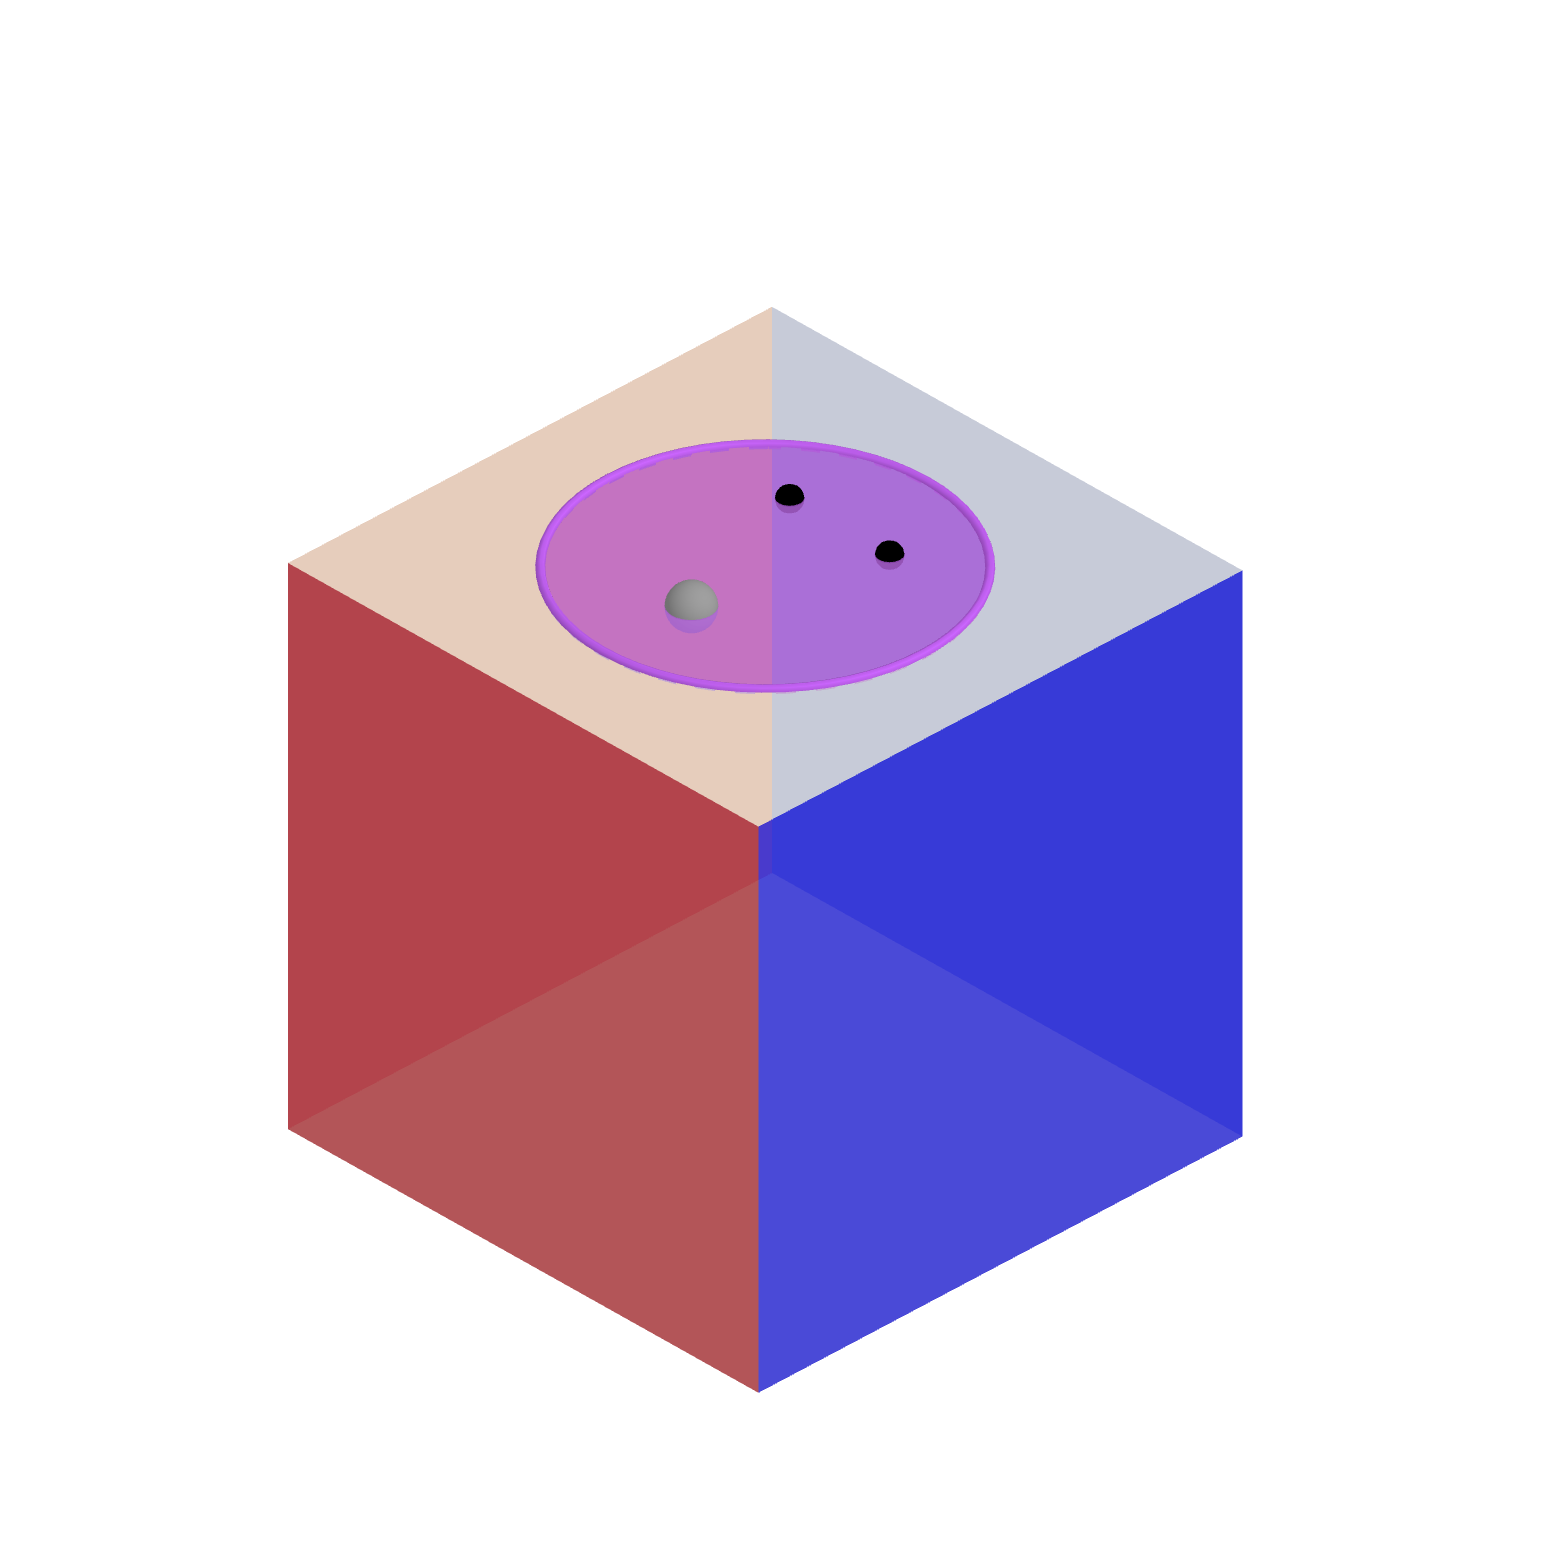
\includegraphics[width=30mm]{figs/curved_cube/curved_cube1}}} \!\!\to\!\! \)
  \( \vcenter{\hbox{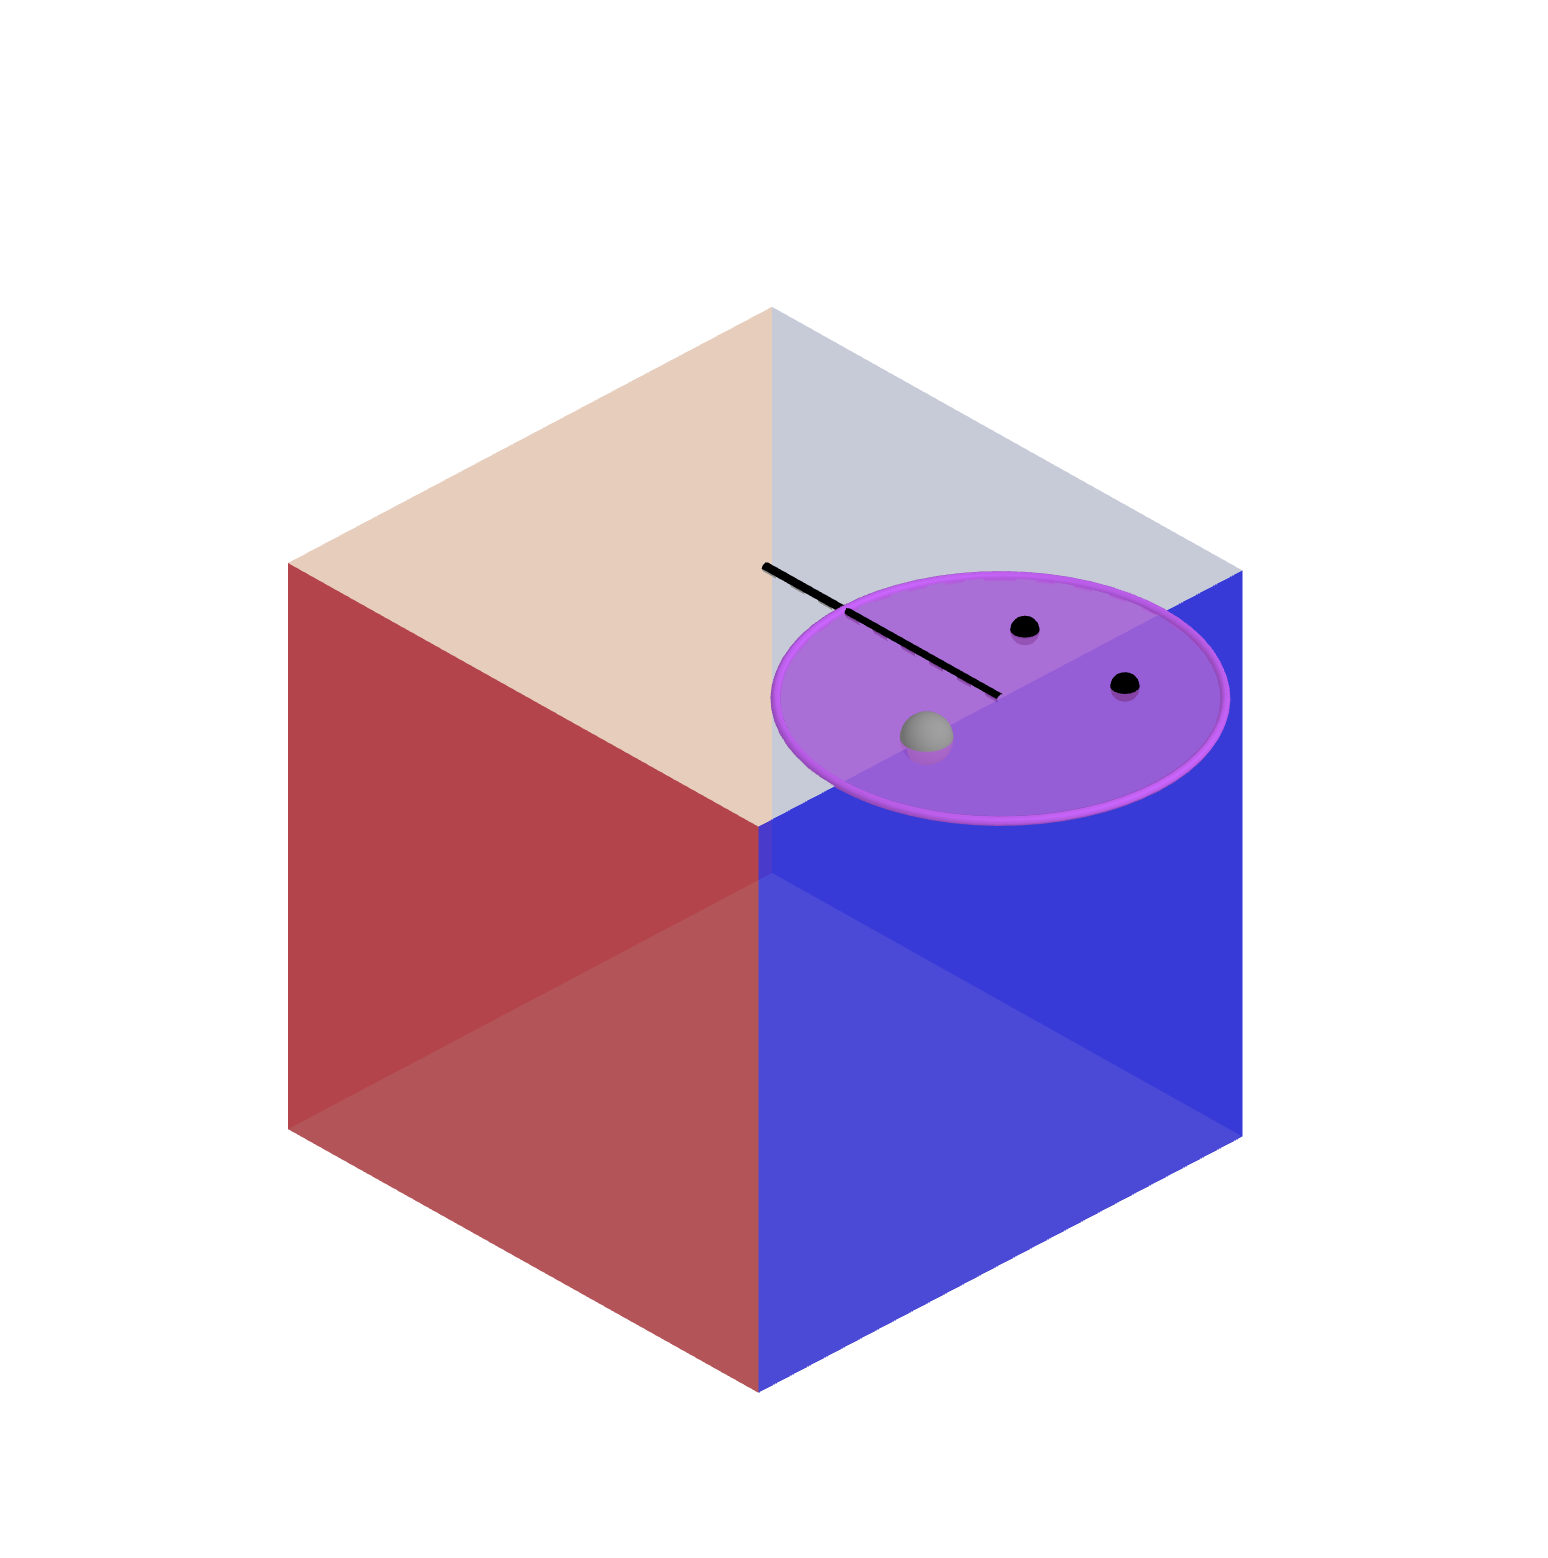
\includegraphics[width=30mm]{figs/curved_cube/curved_cube2}}}\!\!\to\!\! \)
  \( \vcenter{\hbox{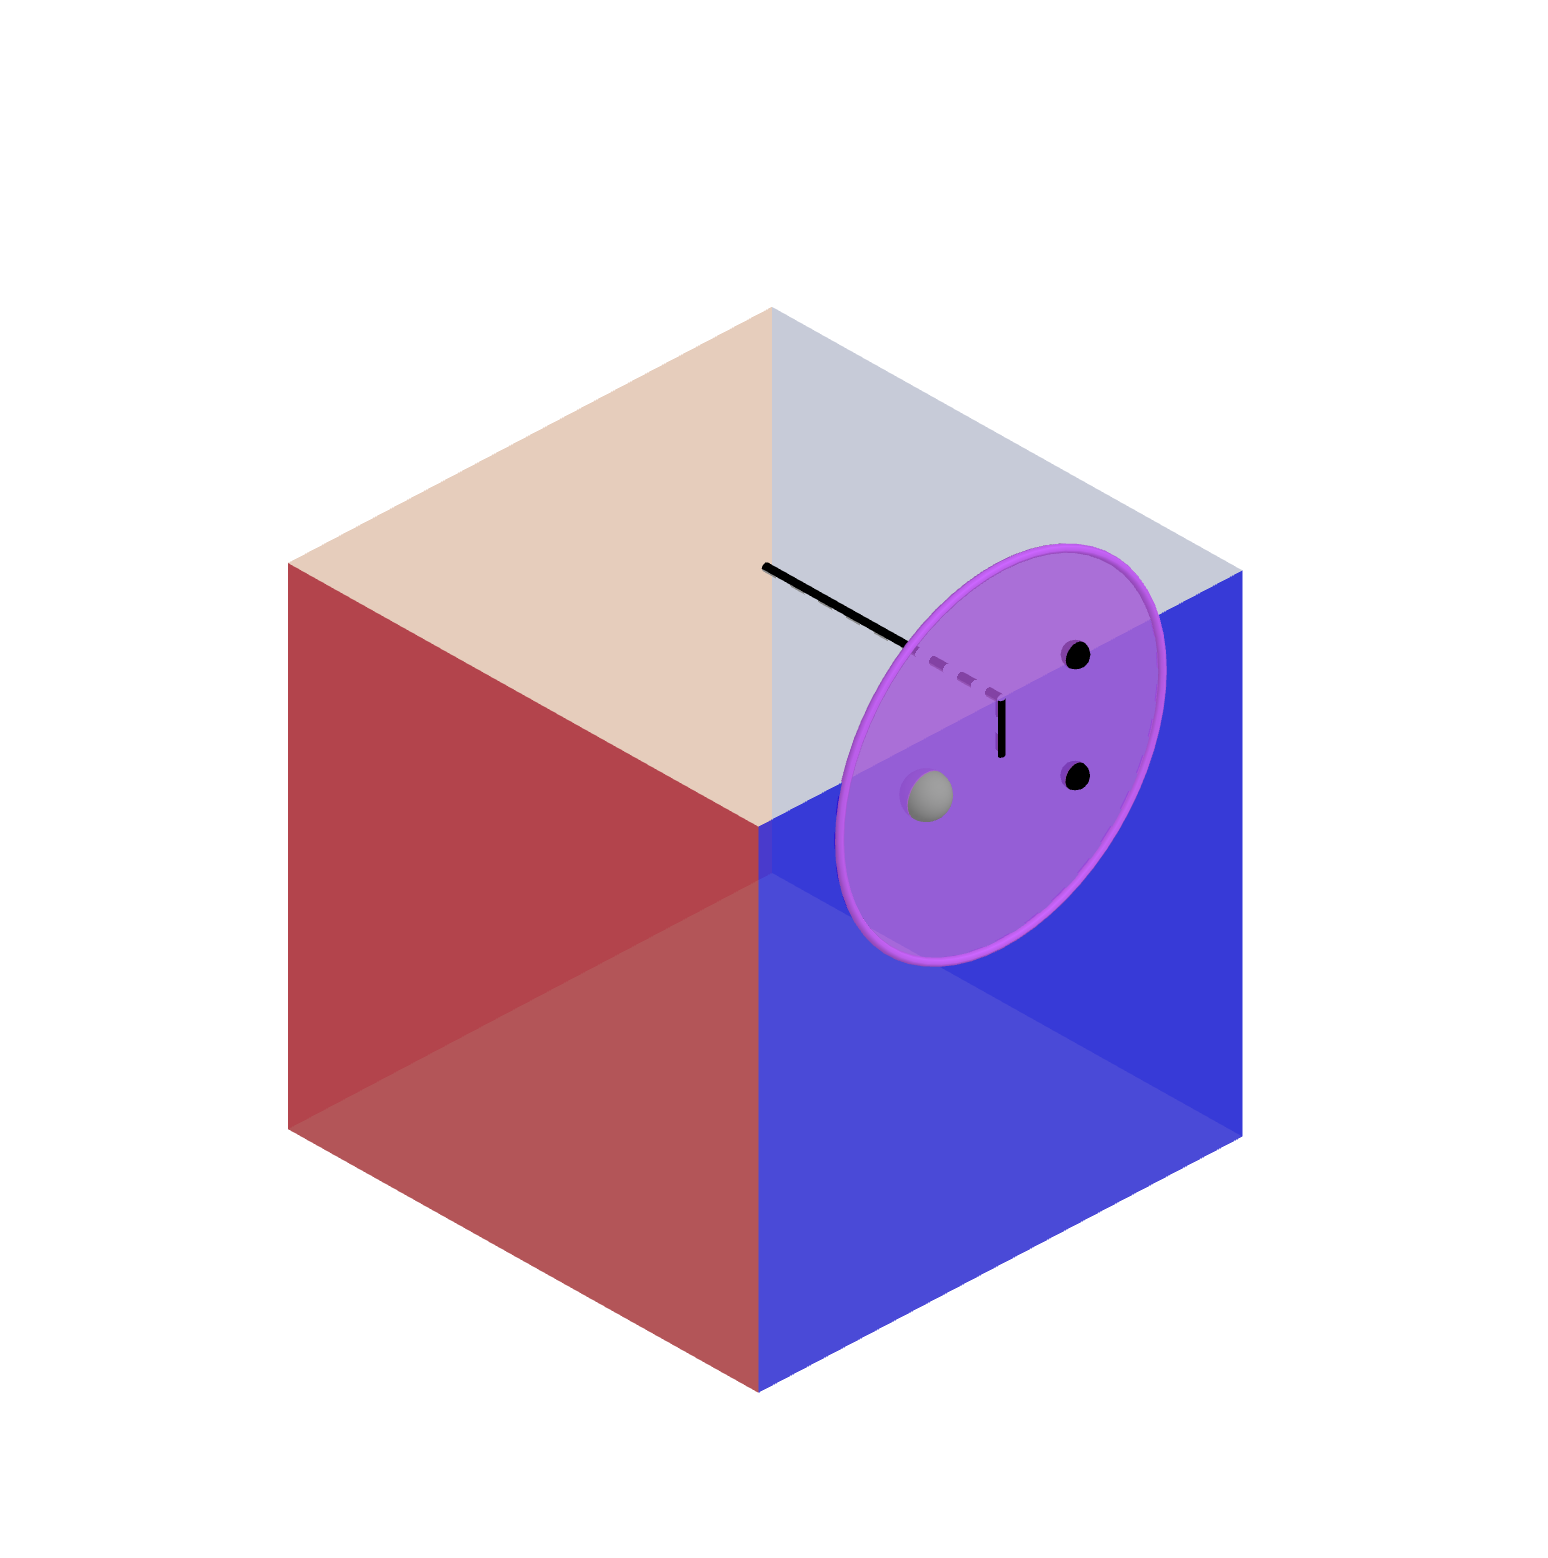
\includegraphics[width=30mm]{figs/curved_cube/curved_cube3}}}\!\!\to\!\! \)
  \( \vcenter{\hbox{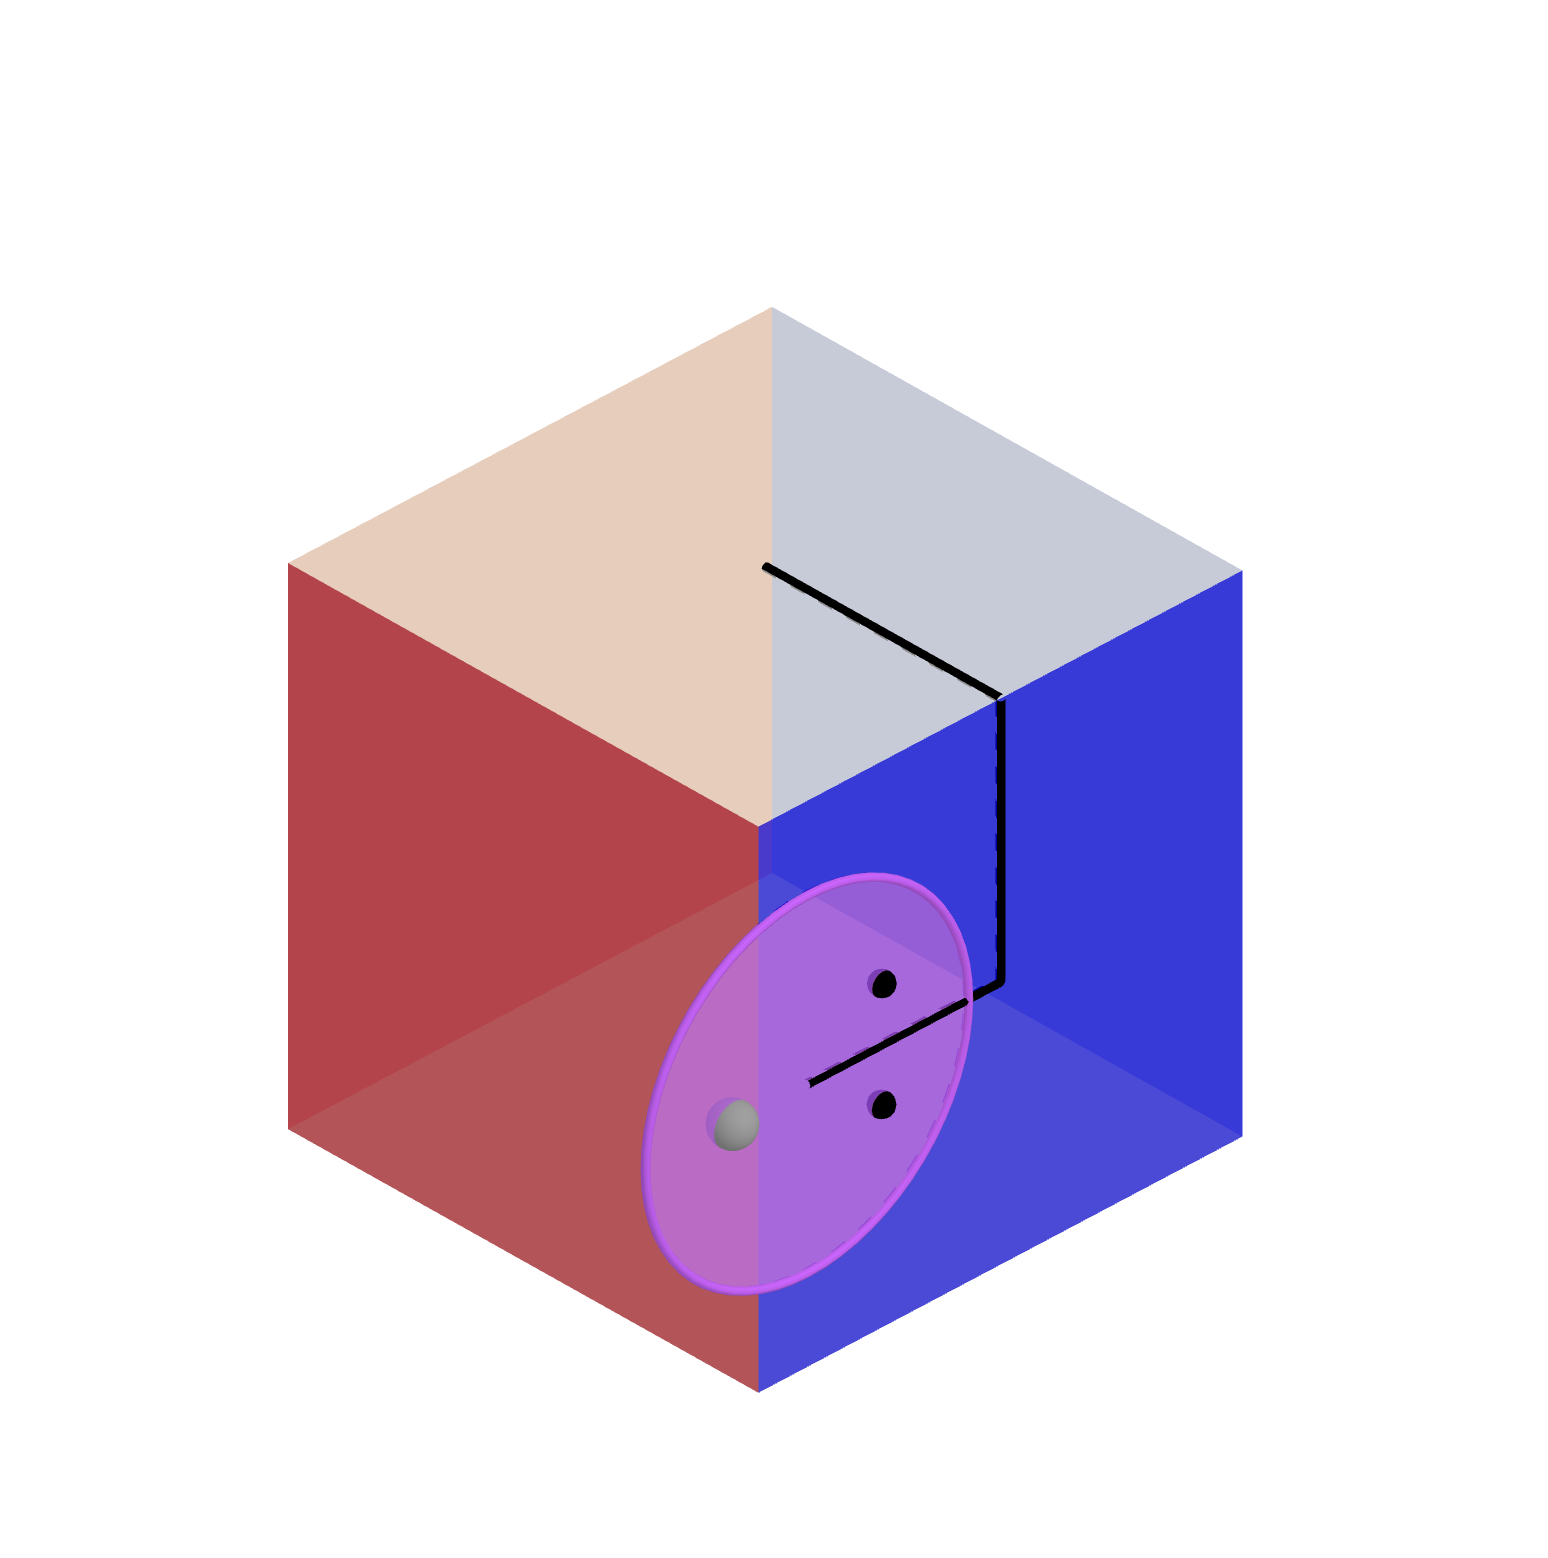
\includegraphics[width=30mm]{figs/curved_cube/curved_cube4}}}\!\!\to\!\! \)
  \( \vcenter{\hbox{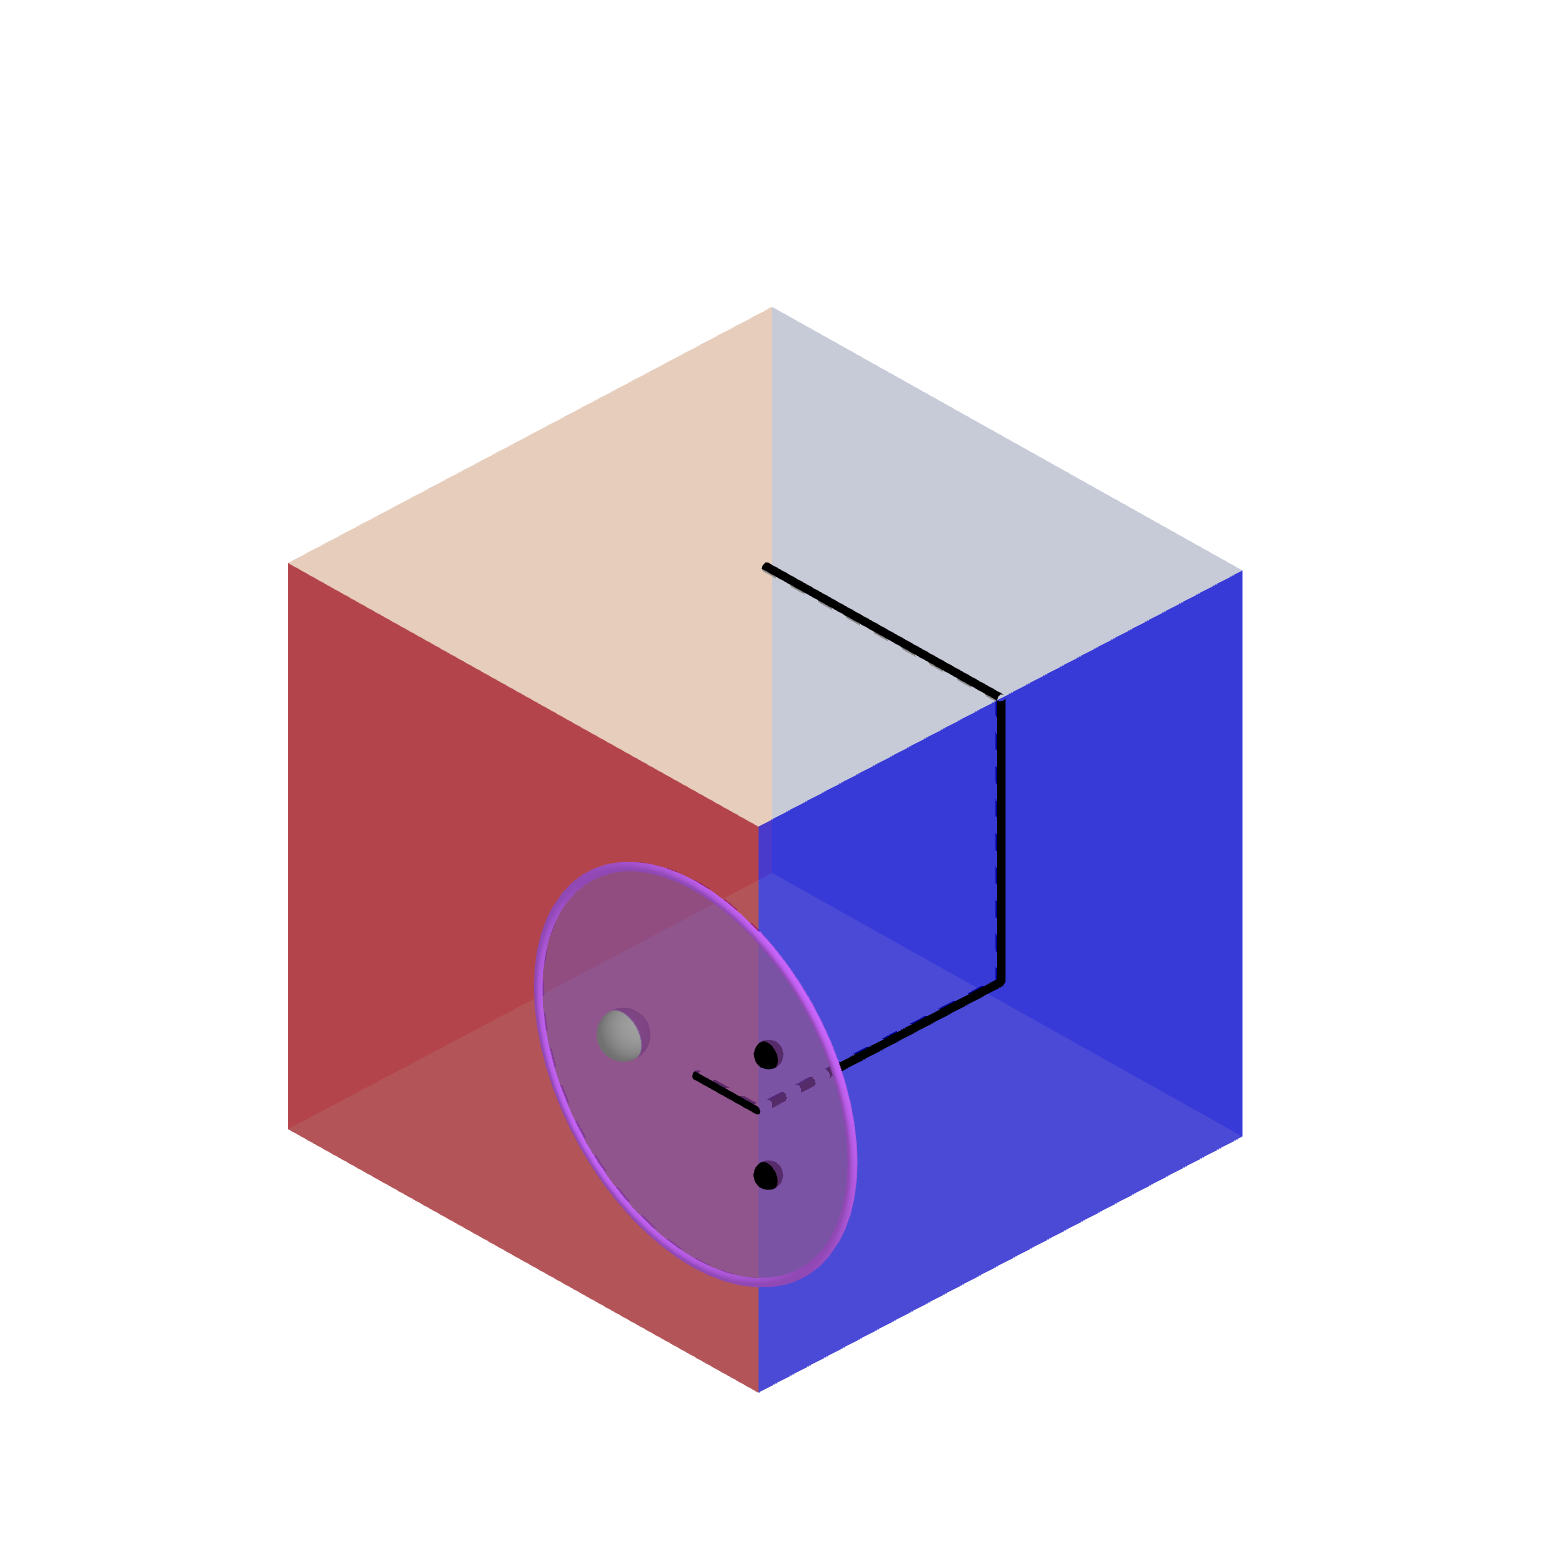
\includegraphics[width=30mm]{figs/curved_cube/curved_cube5}}}\!\!\to\!\! \)
  \( \vcenter{\hbox{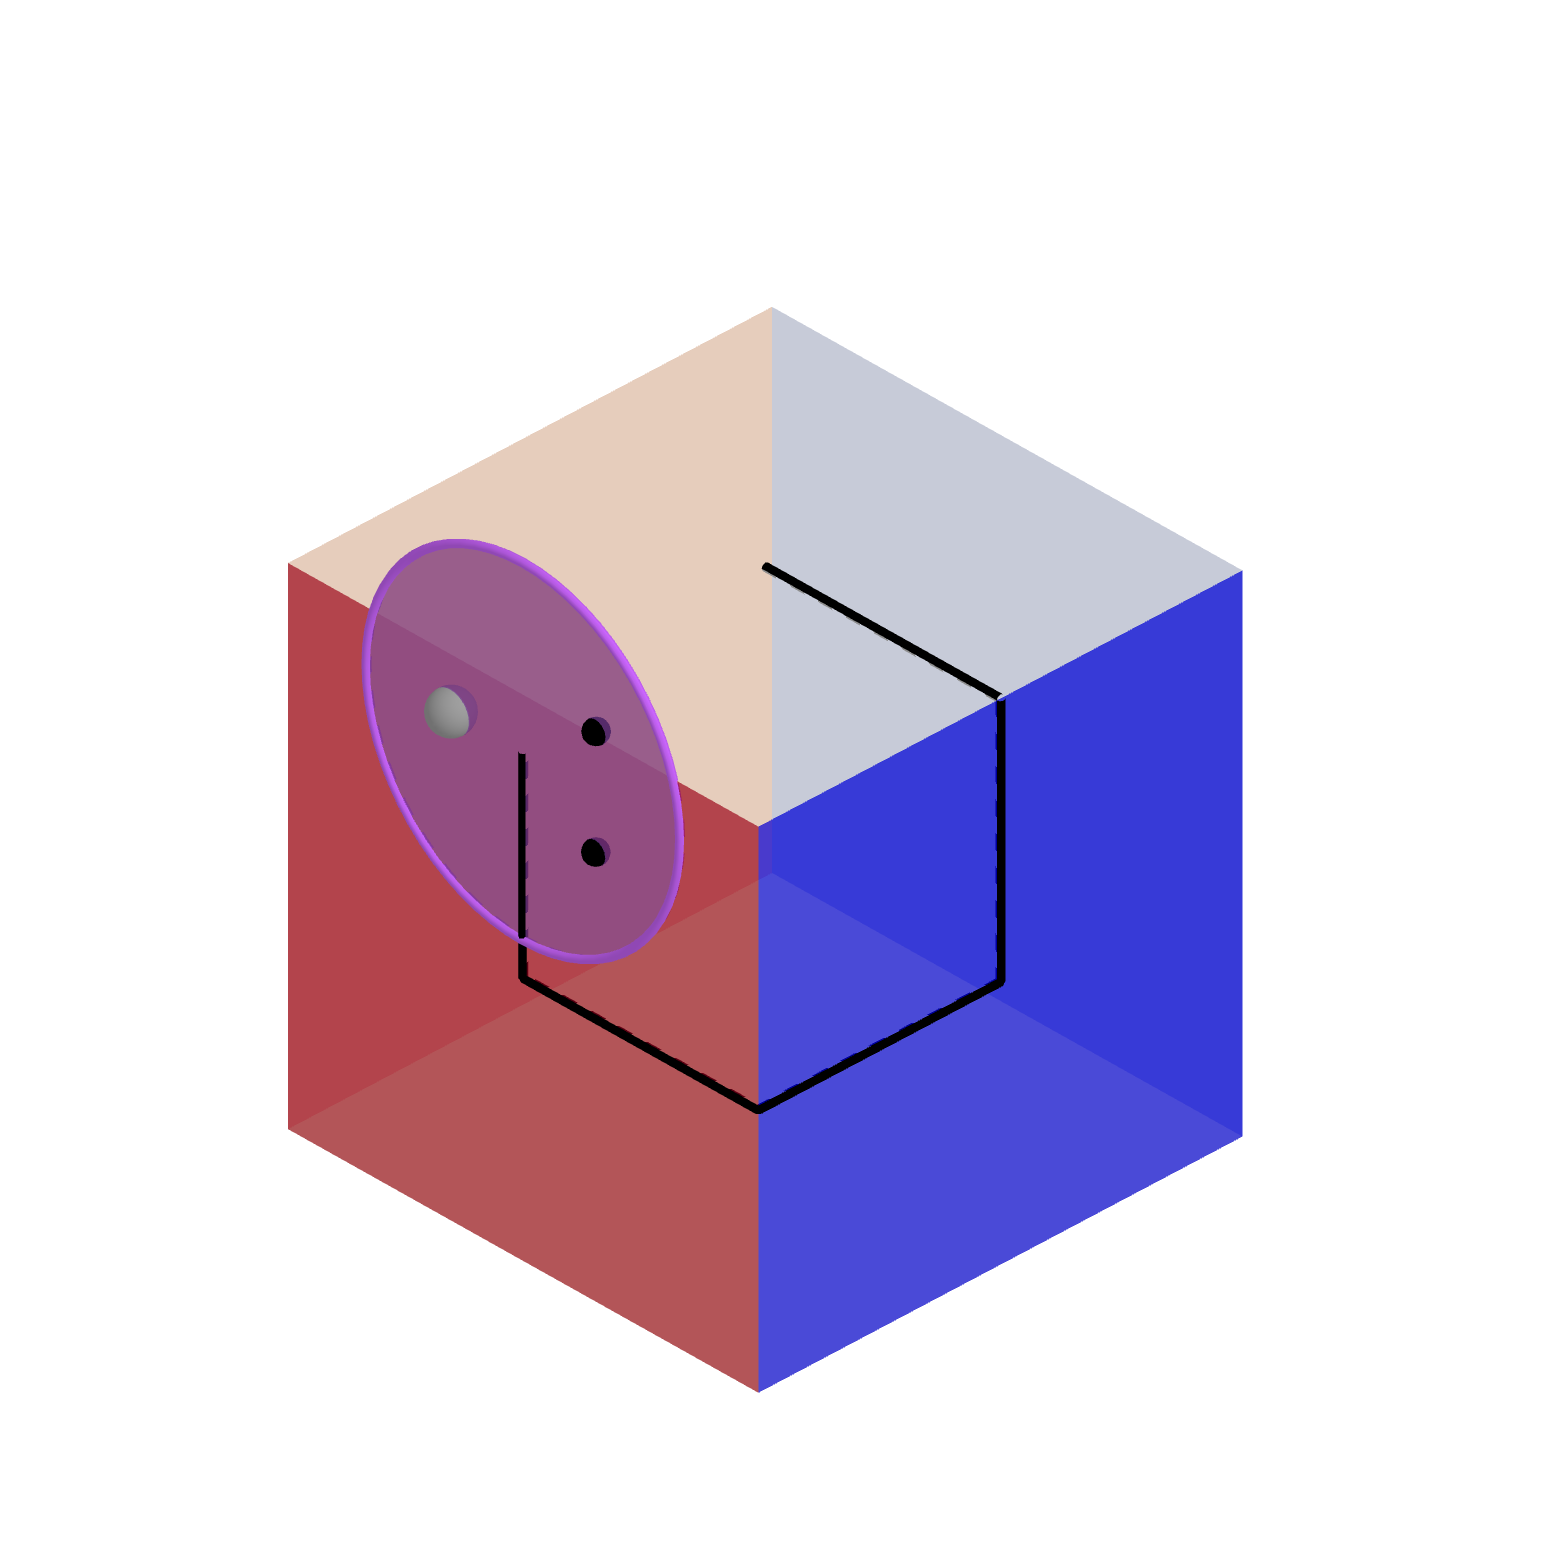
\includegraphics[width=30mm]{figs/curved_cube/curved_cube6}}}\!\!\to\!\! \)
  \( \vcenter{\hbox{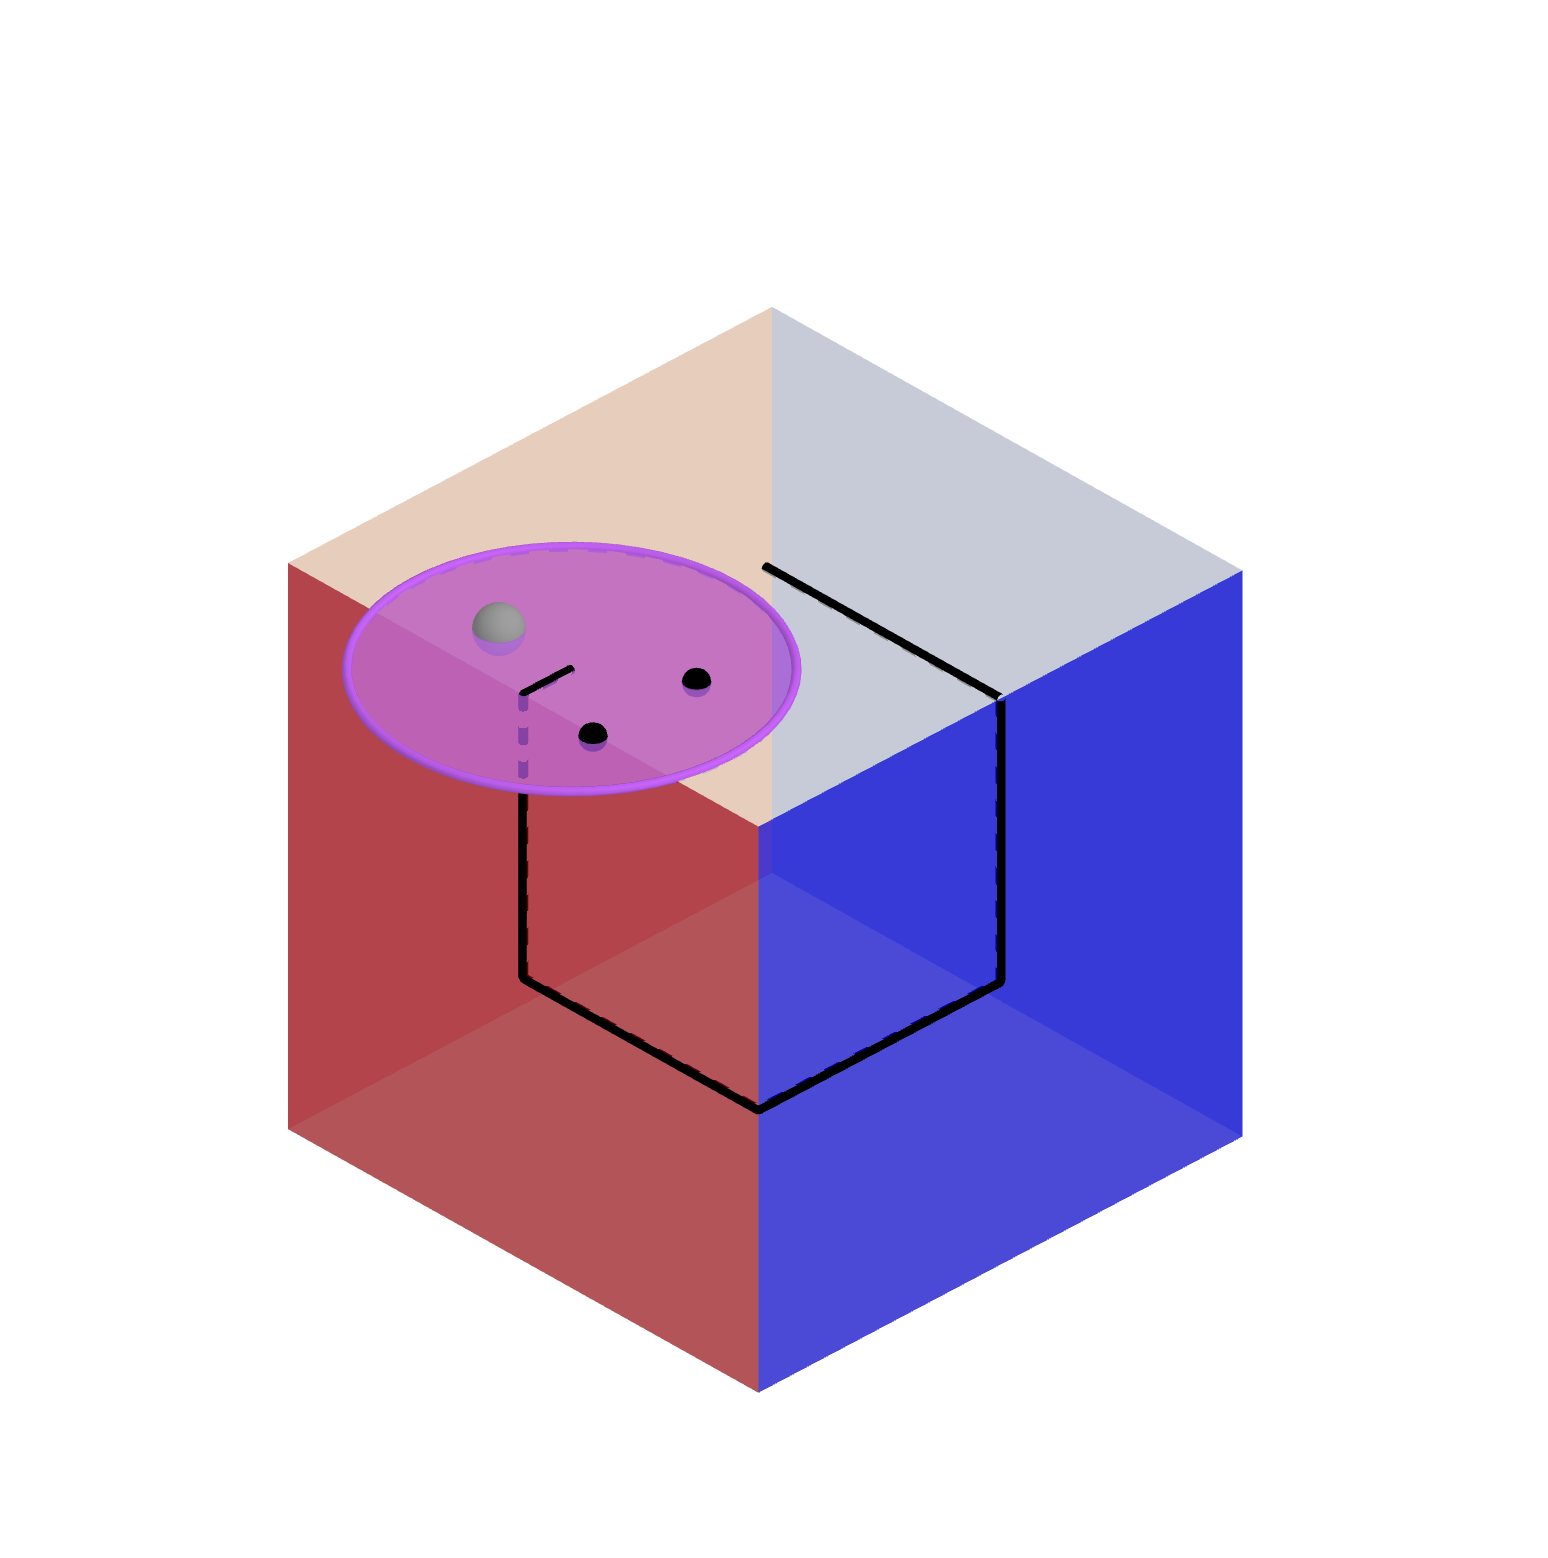
\includegraphics[width=30mm]{figs/curved_cube/curved_cube7}}}\!\!\to\!\! \)
  \( \vcenter{\hbox{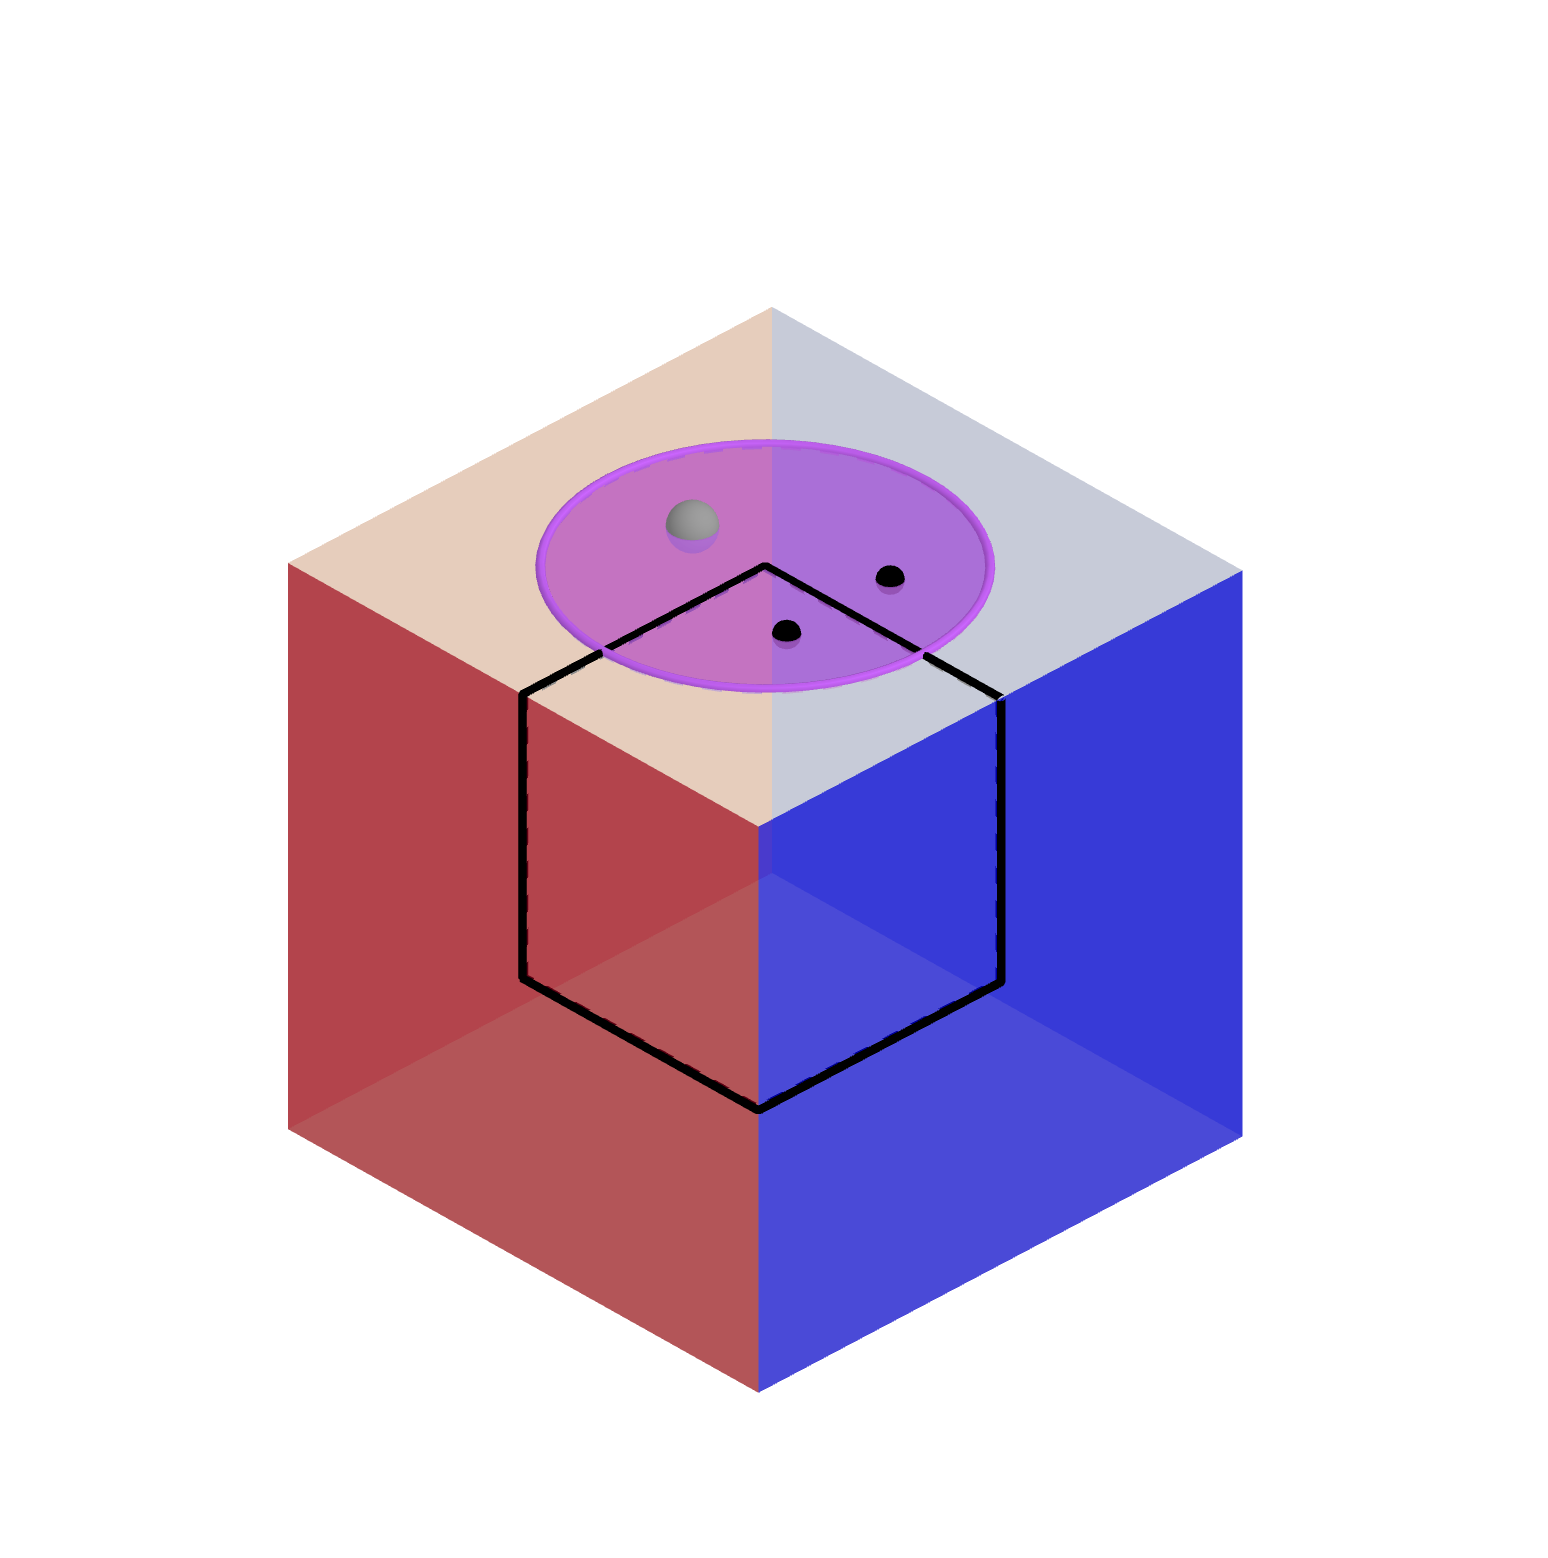
\includegraphics[width=30mm]{figs/curved_cube/curved_cube8}}} \)
\end{frame}

\begin{frame}
Extend \alert{\( \link \)} from vertices to edges of the octahedron, by imagining \alert{tipping}:

\begingroup
\tikzset{every picture/.style={scale=0.85}}
\begin{figure}[h]
\centering
\begin{tikzpicture}%
  [x={(-0.860769cm, -0.121512cm)},
  y={(0.508996cm, -0.205391cm)},
  z={(-0.000053cm, 0.971107cm)},
  scale=1,
  eqback/.style={->, very thick},
  back/.style={loosely dotted, thin},
  eqedge/.style={->, very thick},
  edge/.style={black, thin},
  facet/.style={fill=blue!95!black,fill opacity=0.0},
  vertex/.style={inner sep=1pt,circle,draw=green!25!black,fill=black,thick}]
\coordinate (-1, -1, 0) at (-1, -1, 0);
\coordinate (-1, 1, 0) at (-1, 1, 0);
\coordinate (0, 0, -1) at (0, 0, -1);
\coordinate (0, 0, 1) at (0, 0, 1);
\coordinate (1, -1, 0) at (1, -1, 0);
\coordinate (1, 1, 0) at (1, 1, 0);
%% Drawing edges in the back
%%
\draw[edge,eqback] (-1, -1, 0) -- (-1, 1, 0);
\draw[edge,back] (-1, -1, 0) -- (0, 0, -1.4);
\draw[edge,back] (-1, -1, 0) -- (0, 0, 1.4);
\draw[edge,eqback] (1, -1, 0) -- (-1, -1, 0);
%% Drawing vertices in the back
%%
\node[vertex] at (-1, -1, 0)     {};
%% Drawing the facets
%%
\fill[facet] (1, 1, 0) -- (0, 0, -1.4) -- (1, -1, 0) -- cycle {};
\fill[facet] (1, 1, 0) -- (0, 0, 1.4) -- (1, -1, 0) -- cycle {};
\fill[facet] (1, 1, 0) -- (-1, 1, 0) -- (0, 0, 1.4) -- cycle {};
\fill[facet] (1, 1, 0) -- (-1, 1, 0) -- (0, 0, -1.4) -- cycle {};
%% Drawing edges in the front
%%
\draw[edge] (-1, 1, 0) -- (0, 0, -1.4);
\draw[edge] (-1, 1, 0) -- (0, 0, 1.4);
\draw[eqedge] (-1, 1, 0) -- (1, 1, 0);
\draw[edge] (0, 0, -1.4) -- (1, -1, 0);
\draw[edge] (0, 0, -1.4) -- (1, 1, 0);
\draw[edge] (0, 0, 1.4) -- (1, -1, 0);
\draw[edge] (0, 0, 1.4) -- (1, 1, 0);
\draw[eqedge] (1, 1, 0) -- (1, -1, 0);
%% Drawing the vertices in the front
%%
\begin{scope}[nodes=vertex]
\node[label=above right:\( b \)] at (-1, 1, 0)     {};
\node[label=below:\( y \)] at (0, 0, -1.4)     {};
\node[label=above:\( w \)] at (0, 0, 1.4)     {};
\node[label=above left:\( g \)] at (1, -1, 0)     {};
\node[label=above left:\( r \)] at (1, 1, 0)     {};
\node[label=above right:\( o \)] at (-1, -1, 0)     {};
\end{scope}
\end{tikzpicture}

\begin{tikzpicture}%
  [x={(-0.860769cm, -0.121512cm)},
  y={(0.508996cm, -0.205391cm)},
  z={(-0.000053cm, 0.971107cm)},
  scale=1,
  eqback/.style={->, very thick},
  back/.style={loosely dotted, thin},
  eqedge/.style={->, very thick},
  edge/.style={black, thin},
  facet/.style={fill=blue!95!black,fill opacity=0.0},
  vertex/.style={inner sep=1pt,circle,draw=green!25!black,fill=black,thick}]
\coordinate (-1, -1, 0) at (-1, -1, 0);
\coordinate (-1, 1, 0) at (-1, 1, 0);
\coordinate (0, 0, -1) at (0, 0, -1);
\coordinate (0, 0, 1) at (0, 0, 1);
\coordinate (1, -1, 0) at (1, -1, 0);
\coordinate (1, 1, 0) at (1, 1, 0);
%% Drawing edges in the back
%%
\draw[edge,back] (-1, -1, 0) -- (-1, 1, 0);
\draw[edge,eqback] (-1, -1, 0) -- (0, 0, -1.4);
\draw[edge,eqback] (0, 0, 1.4) -- (-1, -1, 0);
\draw[edge,back] (1, -1, 0) -- (-1, -1, 0);
%% Drawing vertices in the back
%%
\node[vertex] at (-1, -1, 0)     {};
%% Drawing the facets
%%
\fill[facet] (1, 1, 0) -- (0, 0, -1.4) -- (1, -1, 0) -- cycle {};
\fill[facet] (1, 1, 0) -- (0, 0, 1.4) -- (1, -1, 0) -- cycle {};
\fill[facet] (1, 1, 0) -- (-1, 1, 0) -- (0, 0, 1.4) -- cycle {};
\fill[facet] (1, 1, 0) -- (-1, 1, 0) -- (0, 0, -1.4) -- cycle {};
%% Drawing edges in the front
%%
\draw[edge] (-1, 1, 0) -- (0, 0, -1.4);
\draw[edge] (-1, 1, 0) -- (0, 0, 1.4);
\draw[edge] (-1, 1, 0) -- (1, 1, 0);
\draw[edge] (0, 0, -1.4) -- (1, -1, 0);
\draw[eqedge] (0, 0, -1.4) -- (1, 1, 0);
\draw[edge] (0, 0, 1.4) -- (1, -1, 0);
\draw[eqedge] (1, 1, 0) -- (0, 0, 1.4) ;
\draw[edge] (1, 1, 0) -- (1, -1, 0);
%% Drawing the vertices in the front
%%
\begin{scope}[nodes=vertex]
\node[label=above right:\( b \)] at (-1, 1, 0)     {};
\node[label=below:\( y \)] at (0, 0, -1.4)     {};
\node[label=above:\( w \)] at (0, 0, 1.4)     {};
\node[label=above left:\( g \)] at (1, -1, 0)     {};
\node[label=above left:\( r \)] at (1, 1, 0)     {};
\node[label=above right:\( o \)] at (-1, -1, 0)     {};
\end{scope}
\end{tikzpicture}

\begin{tikzpicture}%
  [x={(-0.860769cm, -0.121512cm)},
  y={(0.508996cm, -0.205391cm)},
  z={(-0.000053cm, 0.971107cm)},
  scale=1,
  eqback/.style={->, very thick},
  back/.style={loosely dotted, thin},
  eqedge/.style={->, very thick},
  edge/.style={black, thin},
  facet/.style={fill=blue!95!black,fill opacity=0.0},
  vertex/.style={inner sep=1pt,circle,draw=green!25!black,fill=black,thick}]
\coordinate (-1, -1, 0) at (-1, -1, 0);
\coordinate (-1, 1, 0) at (-1, 1, 0);
\coordinate (0, 0, -1) at (0, 0, -1);
\coordinate (0, 0, 1) at (0, 0, 1);
\coordinate (1, -1, 0) at (1, -1, 0);
\coordinate (1, 1, 0) at (1, 1, 0);
%% Drawing edges in the back
%%
\draw[edge,back] (-1, -1, 0) -- (-1, 1, 0);
\draw[edge,back] (-1, -1, 0) -- (0, 0, -1.4);
\draw[edge,back] (-1, -1, 0) -- (0, 0, 1.4);
\draw[edge,back] (1, -1, 0) -- (-1, -1, 0);
%% Drawing vertices in the back
%%
\node[vertex] at (-1, -1, 0)     {};
%% Drawing the facets
%%
\fill[facet] (1, 1, 0) -- (0, 0, -1.4) -- (1, -1, 0) -- cycle {};
\fill[facet] (1, 1, 0) -- (0, 0, 1.4) -- (1, -1, 0) -- cycle {};
\fill[facet] (1, 1, 0) -- (-1, 1, 0) -- (0, 0, 1.4) -- cycle {};
\fill[facet] (1, 1, 0) -- (-1, 1, 0) -- (0, 0, -1.4) -- cycle {};
%% Drawing edges in the front
%%
\draw[eqedge] (-1, 1, 0) -- (0, 0, -1.4);
\draw[eqedge] (0, 0, 1.4) -- (-1, 1, 0);
\draw[edge] (-1, 1, 0) -- (1, 1, 0);
\draw[eqedge] (0, 0, -1.4) -- (1, -1, 0);
\draw[edge] (0, 0, -1.4) -- (1, 1, 0);
\draw[eqedge] (1, -1, 0) -- (0, 0, 1.4);
\draw[edge] (0, 0, 1.4) -- (1, 1, 0);
\draw[edge] (1, 1, 0) -- (1, -1, 0);
%% Drawing the vertices in the front
%%
\begin{scope}[nodes=vertex]
\node[label=above right:\( b \)] at (-1, 1, 0)     {};
\node[label=below:\( y \)] at (0, 0, -1.4)     {};
\node[label=above:\( w \)] at (0, 0, 1.4)     {};
\node[label=above left:\( g \)] at (1, -1, 0)     {};
\node[label=above left:\( r \)] at (1, 1, 0)     {};
\node[label=above right:\( o \)] at (-1, -1, 0)     {};
\end{scope}
\end{tikzpicture}
\caption{The equators for \( w, b, r \).}
\end{figure}
\endgroup
We obtain \( \tr(\partial(wbr)):Tw=Tw \). 

Extend to the face \( wbr \) via \alert{homotopy} \( \flat(wbr):\id=\tr(\partial(wbr)) \).
\end{frame}

% \begin{frame}{Rotation}
% Let \( R:\gr{abcd}\to\gr{abcd} \) send \( a\mapsto b , b\mapsto c , c\mapsto d, d\mapsto a \). \\~\\
% 
% Extend \( R \) to edges.
% 
% \begin{lemma}
% \( \hgr{R}:\hgr{abcd}\to\hgr{abcd} \) is homotopic to the identity, i.e. we have \( \pit{x:\hgr{abcd}}x=\hgr{R}(x) \).
% \end{lemma}
% \begin{proof}
% Use edges.
% \end{proof}
% \end{frame}

\begin{frame}
\begin{definition}
If \( \mm\defeq \mm_0\xrightarrow[]{\imath_0}\cdots\xrightarrow[]{\imath_{n-1}}\mm_n \) is a cellular type and all the triangles commute in the diagram:\vspace{-10pt}
\[\begin{tikzcd}[ampersand replacement=\&, column sep=small]
  {\mm_0} \& {\mm_1} \& {\mm_2} \& \cdots \& {\mm_n} \\
\&\& {\mathcal{U}}
\arrow["{\imath_0}", from=1-1, to=1-2]
\arrow["{f_0}", from=1-1, to=2-3]
\arrow["{\imath_1}", from=1-2, to=1-3]
\arrow["{f_1}", from=1-2, to=2-3]
\arrow["{\imath_2}", from=1-3, to=1-4]
\arrow["{f_2}", from=1-3, to=2-3]
\arrow["{\imath_{n-1}}", from=1-4, to=1-5]
\arrow["f_n"', from=1-5, to=2-3]
\end{tikzcd}\]\vspace{-15pt}
\begin{itemize}
\item The map \( f_k \) is a \defemph{\( k \)-bundle} on \( \mm \).
\item The pair given by the map \( f_k \) and the proof \( f_k\circ \imath_{k-1}=f_{k-1} \), i.e. that \( f_k \) extends \( f_{k-1} \) is called a \defemph{\( k \)-connection on the \( (k-1) \)-bundle \( f_{k-1} \)}.
\end{itemize}
\end{definition}
\end{frame}

\begin{frame}
\begin{mydef}
\[\begin{tikzcd}[ampersand replacement=\&, column sep=small]
  {M_k\times \partial\Delta^k} \& {M_k} \\
  {\mathbb{M}_{k-1}} \& {\mathbb{M}_k} \\
  \& {\mathcal{U}}
  \arrow["{\mathrm{pr}_1}", from=1-1, to=1-2]
  \arrow["{\mathbb{A}_{k-1}}"', from=1-1, to=2-1]
  \arrow["{*_{\mathbb{M}_k}}", from=1-2, to=2-2]
  \arrow["{h_k}", shorten <=10pt, shorten >=10pt, Rightarrow, from=2-1, to=1-2]
  \arrow["{\imath_{k-1}}", from=2-1, to=2-2]
  \arrow[""{name=0, anchor=center, inner sep=0}, "{f_{k-1}}"', from=2-1, to=3-2]
  \arrow["\ulcorner"{pos=-0.05, rotate=180}, shift left=1.5, draw=none, from=2-2, to=1-1]
  \arrow["{f_k}", from=2-2, to=3-2]
  \arrow[shorten >=3pt, Rightarrow, from=2-2, to=0]
\end{tikzcd}
\begin{tikzcd}[ampersand replacement=\&]
  {\{m_k\}\times \partial\Delta^k} \& \unit \\
  {\mathbb{M}_{k-1}} \& {\mathcal{U}}
  \arrow["{!}", from=1-1, to=1-2]
  \arrow["{\mathbb{A}_{k-1}}"', from=1-1, to=2-1]
  \arrow["{*_{\mathbb{M}_k}}", from=1-2, to=2-2]
  \arrow["{\flat_k}", shorten <=11pt, shorten >=11pt, Rightarrow, from=1-2, to=2-1]
  \arrow[from=2-1, to=2-2]
\end{tikzcd}\]
the filler \( \flat_k \) is called a \defemph{flatness structure for the face \( m_k \)}, and its ending path is called \defemph{curvature at the face \( m_k \)}.
\end{mydef}
\end{frame}

\section{Vector fields}
\begin{frame}{Vector fields}
\begin{columns}
\begin{column}{0.7\textwidth}
Let \( T:\mm_2\to\Kzt \) be an oriented tangent bundle on an oriented 2-dim cellular type
\begin{itemize}
\item A \alert{vector field} is a term \( X:\pit{m:\mm_1}Tm \).
\item It's a \alert{nonvanishing} vector field on the 1-skeleton.
\item We model classical zeros by omitting the faces.
\end{itemize}
\end{column}
\begin{column}{0.3\textwidth}
\begin{tikzpicture}%
  [x={(-0.860769cm, -0.121512cm)},
  y={(0.508996cm, -0.205391cm)},
  z={(-0.000053cm, 0.971107cm)},
  scale=1,
  back/.style={loosely dotted, thin},
  edge/.style={black, thick},
  arrow/.style={black, very thick, solid, -{Stealth[scale=0.8]}},
  facet/.style={fill=blue!95!black,fill opacity=0.0},
  vertex/.style={inner sep=1pt,circle,draw=green!25!black,fill=black,thick}]
%% Drawing the vertices in the front
%%
\begin{scope}[nodes=vertex]
\node[label=above right:\( b \)] at (-1, 1, 0) (b)     {};
\node[label=below:\( y \)] at (0, 0, -1.4) (y)    {};
\node[label=above:\( w \)] at (0, 0, 1.4)  (w)   {};
\node[label=above left:\( g \)] at (1, -1, 0) (g)    {};
\node[label=above left:\( r \)] at (1, 1, 0)  (r)   {};
\node[label=above right:\( o \)] at (-1, -1, 0) (o)    {};
\end{scope}
%% Drawing edges in the back
%%
\draw[edge,back,arrow] (o) -- (b);
\draw[edge,back,arrow] (y) -- (o);
\draw[edge,back] (o) -- (w);
\draw[edge,back] (o) -- (g);
%% Drawing vertices in the back
%%
\node[vertex] at (o)     {};
%% Drawing the facets
%%
\fill[facet] (1, 1, 0) -- (0, 0, -1.4) -- (1, -1, 0) -- cycle {};
\fill[facet] (1, 1, 0) -- (0, 0, 1.4) -- (1, -1, 0) -- cycle {};
\fill[facet] (1, 1, 0) -- (-1, 1, 0) -- (0, 0, 1.4) -- cycle {};
\fill[facet] (1, 1, 0) -- (-1, 1, 0) -- (0, 0, -1.4) -- cycle {};
%% Drawing edges in the front
%%
\draw[edge,arrow] (b) -- (y);
\draw[edge] (b) -- (w);
\draw[edge] (b) -- (r);
\draw[edge] (y) -- (g);
\draw[edge] (y) -- (r);
\draw[edge,arrow] (g) -- (w);
\draw[edge,arrow] (w) -- (r);
\draw[edge,arrow] (r) -- (g);
\end{tikzpicture}

\end{column}
\end{columns}
\end{frame}

\begin{frame}
\begin{columns}
\begin{column}{0.6\textwidth}
\vspace{12pt}
\begingroup
\tikzset{every picture/.style={scale=0.85}}
\begin{tikzpicture}
  [arrow/.style={-{Stealth[scale=1.1]}}, vec/.style={ultra thick, color=black}, vectr/.style={thick, color=black}, vectrtr/.style={thick, dashed, color=black}, vectrtrtr/.style={thick, dotted, color=black}]
  \tikzset{oo/.style={circle, scale=0.6, fill=black}}
  \tikzset{ii/.style={circle, scale=0.3, fill=gray}}
  \setlength{\mylen}{3cm}
  \setlength{\mylin}{1.2cm}
    \node[oo, label=below right:\( v_1 \)] (V1) at (0, 0) {};
    \node[oo, label=below:\( v_3 \)] (V3) at (2*\mylen, 0) {};
    \node[oo, label=above:\( v_2 \)] (V2) at (\mylen, 1.732*\mylen) {};

    \draw[arrow] (V2) edge[very thick, color=teal, "\( e_{23} \)"] (V3);
    \draw[arrow] (V1) edge[very thick, color=magenta, "\( e_{12} \)"] (V2);
    \draw[arrow] (V3) edge[very thick, color=blue, "\( e_{31} \)"] (V1);
    
    \node [ii, above right=\mylin of V1] (V11) {};
    \node [ii, below right=\mylin of V1] (V14) {};
    \node [ii, below left=\mylin of  V1] (V13) {};
    \node [ii, above left= \mylin of V1] (V12) {};

    \node [left=1.3\mylin of  V1,  label=center:\( T_1 \)] {};
    \node [right=1.3\mylin of  V2,  label=center:\( T_2 \)] {};
    \node [right=1.3\mylin of  V3,  label=center:\( T_3 \)] {};

    \node [ii, above right=\mylin of V2] (V21) {};
    \node [ii, below right=\mylin of V2] (V24) {};
    \node [ii, below left=\mylin of  V2] (V23) {};
    \node [ii, above left= \mylin of V2] (V22) {};

    \node [ii, above right=\mylin of V3] (V31) {};
    \node [ii, below right=\mylin of V3] (V34) {};
    \node [ii, below left=\mylin of  V3] (V33) {};
    \node [ii, above left= \mylin of V3] (V32) {};

    \draw[dashed] (V11) -- (V12);
    \draw[dashed] (V12) -- (V13);
    \draw[dashed] (V13) -- (V14);
    \draw[dashed] (V14) -- (V11);

    \draw[dashed] (V21) -- (V22);
    \draw[dashed] (V22) -- (V23);
    \draw[dashed] (V23) -- (V24);
    \draw[dashed] (V24) -- (V21);
    
    \draw[dashed] (V31) -- (V32);
    \draw[dashed] (V32) -- (V33);
    \draw[dashed] (V33) -- (V34);
    \draw[dashed] (V34) -- (V31);
    
    \draw[arrow] (V1) edge[vec] (V11);
    \draw[arrow] (V2) edge[vectr] (V21);
    \draw[arrow] (V3) edge[vectrtr] (V34);
    \draw[arrow] (V1) edge[vectrtrtr] (V14);

    \draw[arrow] (V2) edge[vec] (V24);
    \draw[arrow] (V3) edge[vectr] (V33);
    \draw[arrow] (V1) edge[vectrtr] (V13);

    \draw[arrow] (V21) edge[thick, color=magenta] (V24);
    \draw[arrow] (V34) edge[thick, color=magenta] (V33);
    \draw[arrow] (V14) edge[thick, color=magenta] (V13);
    \draw[arrow] (V33) edge[thick, color=teal] (V32);
    \draw[arrow] (V13) edge[thick, color=teal] (V12);
    \draw[arrow] (V12) edge[thick, color=blue] (V11);

    \draw[arrow] (V3) edge[vec] (V32);
    \draw[arrow] (V1) edge[vectr] (V12);
\end{tikzpicture}

\endgroup
\end{column}
\begin{column}{0.4\textwidth}
\begin{itemize}
\item \( \partial F\defeq e_{12}\cdot e_{23}\cdot e_{31}  \)
\item We access pathovers asymmetrically: \( X_{12}:T_{12}X_1=_{T_2}X_2 \)
\item \( X(\partial F) \) is 3-sided inside a square
\item To make a loop we cat with \( \flat(\partial F) \)
\end{itemize}
\end{column}
\end{columns}
\end{frame}

\begin{frame}
\[\begin{aligned}
\tr_F&\defeq \tr(\partial F)&&:Tm=Tm&&\text{\alert{holonomy}}\\
\flat_F&\defeq \flat(\partial F)&&:\id=_{Tm=Tm}\tr(\partial F)&&\text{\alert{flatness}}\\
X_F&\defeq X(\partial F)&&:\tr(\partial F)(X(m))=_{Tm}X(m)&&\text{\alert{swirling}}\\
\end{aligned}\]
\onslide<2->{
\begin{columns}[c]
\begin{column}{0.7\textwidth}
\begin{mydef}
The \defemph{index of the vector field \( X \) on the face \( F \)} is the integer \( I^X_F\defeq\loopy(\flat_F(X(m))\cdot X_F):\loopy(X(m)=_{Tm}X(m)) \).
\end{mydef}
\end{column}
\begin{column}{0.3\textwidth}
\begin{tikzpicture}
  [arrow/.style={-{Stealth[scale=1.1]}}, .style={scale=0.7}]
  \tikzset{oo/.style={circle, scale=0.6, fill=black}}
  \tikzset{ii/.style={circle, scale=0.3, fill=gray}}
  \setlength{\mylen}{2cm}
  \setlength{\mylin}{1cm}
  \node[label=center:\( Tv_1 \)] (V1) at (0, 0) {};
  \node [ii, above right=\mylin of V1,  label=right:\( v_{11} \)] (V11) {};
  \node [ii, below right=\mylin of V1,  label=right:\( v_{12} \)] (V12) {};
  \node [ii, below left=\mylin of  V1,  label=left:\( v_{13} \)] (V13) {};
  \node [ii, above left= \mylin of V1,  label=left: \( v_{14} \)] (V14) {};

  \draw[dashed] (V11) edge[ultra thick, solid, arrow, swap, "\( \flat_F(X_1) \)"] (V14);
  \draw[arrow] (V14) edge[thick, swap, color=magenta, "\( X_{12} \)"] (V13);
  \draw[arrow] (V13) edge[thick, swap, color=teal, "\( X_{23} \)"] (V12);
  \draw[arrow] (V12) edge[thick, swap, color=blue, "\( X_{31} \)"] (V11);
\end{tikzpicture}
\end{column}
\end{columns}}
\end{frame}

\section{Results}

\begin{frame}
How do we make these happen?
\begin{align*}
\sum_F \flat_F &\leftrightsquigarrow \int_M K\,dA  \\
\sum_F I^X_F &\leftrightsquigarrow  \sum_{i=1}^{n} \mathsf{index}_{x_i} \\
? &\leftrightsquigarrow \frac{1}{2\pi}\int_M K\,dA + \sum_{i=1}^{n} \mathsf{index}_{x_i} = 0 
\end{align*}
\end{frame}

\begin{frame}
\onslide<1->{Observation 1: Use the torsor structure. If we choose \( m:\mm \) then \( T_m=T_m \) acts on all fibers. We can define subtraction \( T_i\times T_i\to(T_m=T_m) \).}

\onslide<2->{Observation 2: Use the vector field. Given \( X_i:T_i \) we can form subtraction \( -X_i:T_i\to (T_m=T_m) \). \( X_{ij}-X_j:T_{ji}X_i-X_j=_{T_m=T_m}0 \).}

\onslide<3->{Observation 3: Use \( \ap \) of addition. We can add \( \alpha:a=_{\ccc(4)}0 \) and \( \beta:b=_{\ccc(4)}0 \) to form \( \alpha+\beta:(a+b)=_{\ccc(4)}0 \).}

\onslide<4->{Together these remove the dependency. We can compute \( \flat, I, X \) on each face independently and total them in \( T_m=T_m \).}
\end{frame}

\begin{frame}{Classical proof}
\begin{columns}
\column{0.5\textwidth}
\vspace{12pt}
\begin{figure}
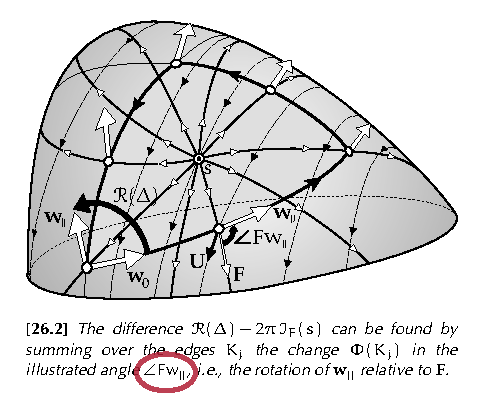
\includegraphics[width=0.9\textwidth]{figs/needham_triangle_circ.pdf}
\caption{{Needham,~T. (2021) Visual Differential Geometry and Forms.}}
\end{figure}
\column{0.5\textwidth}
\vspace{-12pt}
\begin{itemize}
\item The classical proof is discrete-flavored.
\item ``\( \angle Fw_{||} \)'' looked a lot like a pathover.
\item Hopf's \( \Phi \) is defined on edges, not loops. We imitated that too.
\end{itemize}
\end{columns}
\end{frame}


\begin{frame}
Thank you.
\end{frame}

\end{document}
